%%%%%%%%%%%%%%%%%%%%%%%%%%%%%%%%%%%%%%%%%%%%%%%%%%%%%%%%%%%%%%%%%%%%%%%%%%%%%%%%
% > Лабораторная работа 7: Поперечные колебания круглой пластины.
% > Баталов Семен, Антонова Мария, Клюшин Максим, Хайретдинова Диана.
% > 2021 год.
%%%%%%%%%%%%%%%%%%%%%%%%%%%%%%%%%%%%%%%%%%%%%%%%%%%%%%%%%%%%%%%%%%%%%%%%%%%%%%%%

\documentclass[12pt, a4paper]{article}
\usepackage[left=2cm, right=2cm, top=2.5cm, bottom=2.5cm, nohead, 
footskip=1cm]{geometry}
\usepackage{graphicx}
\graphicspath{{./Pictures/}}
\usepackage[utf8]{inputenc}
\usepackage[english, russian]{babel}
\usepackage{indentfirst}
\usepackage{array}
\usepackage{longtable}
\usepackage{misccorr}
\usepackage{setspace, amsmath}
\usepackage{multirow}
\usepackage{subcaption}


\begin{document}
    
    \newcolumntype{M}[1]{>{\centering\arraybackslash}m{#1}}
    \renewcommand{\arraystretch}{1.4}
    
    \begin{center}
        \large{Санкт-Петербургский государственный университет} \\
        \large{Saint-Petersburg State University}\\
        \hfill \break
        \hfill \break
        \hfill \break
        \hfill \break
        \hfill \break
        \hfill \break
        \hfill \break
        \large{Кафедра теоретической и прикладной механики} \\
        \hfill \break
        \hfill \break
        \large{\textbf{ОТЧЕТ}} \\
        \large{\textbf{По лабораторной работе 7}} \\
        \large{<<Поперечные колебания круглой пластины>>} \\
        \hfill \break
        \hfill \break
        \hfill \break
        \large{По дисциплине} \\
        \large{<<Лабораторный практикум по теоретической механике>>} \\
    \end{center}
    
    \hfill \break
    \hfill \break
    \hfill \break
    \hfill \break
    \hfill \break
    \hfill \break
    
    \begin{flushright} 
        \large{Выполнили:} \\
        \hfill \break
        \large{Баталов С. А.} \\
        \large{Антонова М. Н.} \\
        \large{Клюшин М. А.} \\
        \large{Хайретдинова Д. Д.} \\
    \end{flushright}
    
    \hfill \break
    \hfill \break
    \hfill \break
    \hfill \break
    
    \begin{center} 
        \large{Санкт-Петербург} \\
        \large{2021} \\
    \end{center}
    
    \thispagestyle{empty}
    \newpage
    \sloppy
    
    \section{Описание установки}
    
    В этой лабораторной работе анализируются поперечные колебания круглой упругой пластины. Целью работы является экспериментальное определение собственных частот поперечых колебаний упругой пластины, наблюдение соответствующих собственных форм колебаний и сравнение экспериментально определенных собственных частот с их расчетными значениями. В процессе исследовая формы колебаний определяются с помощью фигур Хладни.
    
    \begin{figure} [h]
        \centering
        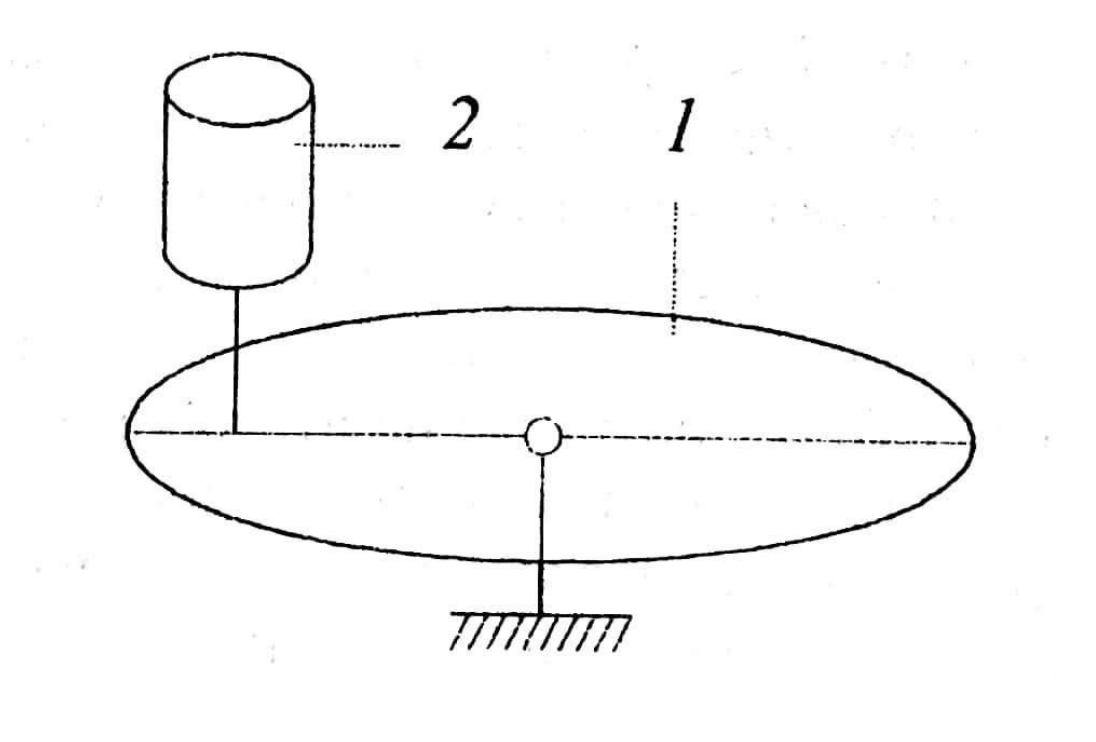
\includegraphics [width = 13cm] {Lab_7_1.png}
        \caption{\centering Схема лабораторной установки.}
        \label{im1}
    \end{figure}
    
    3кспериментальная установка, показанная на рис.~\ref{im1}, представляет собой круглую упругую пластину \textit{1}, жестко закрепленную по краям центрального отверстия и свободную на внешнем крае. К пластине присоединена тяга электромагнита \textit{2}, питаемого переменным током звуковой частоты от генератора. Электромагнит предназначен для создания периодической возмущающей силы, прикладываемой к пластине, частота возмущающей силы равна частоте переменного тока.
    
    \newpage
    
    \section{Параметры установки}
    
    В следующей таблице представлены заранее известные параметры установки: плотность материала пластины~--~$\rho$, коэффициент Пуассона~--~$\sigma$, модуль упругости~--~$E$, толщина пластины~--~$h$, внешний радиус пластины~--~$R$, диаметр внутреннего отверстия~--~$d$.
    
    \begin{longtable}{| M{2cm} | M{3cm} | M{3cm} | M{3cm} |}
        \caption{\centering Известные параметры.}
        \label{tb1} \\
        \hline
        Номер & Величина & Значение & Размерность \\
        \hline
        1 & $\rho$ & 2850 & $\text{кг} / \text{м}^{3}$ \\
        2 & $\sigma$ & 0,5 & -- \\
        3 & $E$ & $7 \cdot 10^{10}$ & Па \\
        \hline
        4 & $h$ & 0,003 & м \\
        5 & $R$ & 0,240 & м \\
        6 & $d$ & 0,008 & м \\
        \hline
    \end{longtable}
    
    \newpage
    
    \section{Теоретические исследования}
    
    Собственная форма колебаний однородной пластины подчиняется дифференциальному
    уравнению (\ref{eq1}), записанному в полярных координатах $(r, \, \phi)$.
    
    \begin{equation}
        \begin{aligned}
        \Delta(\Delta w(r, \, \phi)) - \frac{\rho h p^{2}}{D}w(r, \, \phi) = 0, \quad \text{где} \\
        \Delta = \frac{\partial^{2}}{\partial r^{2}} + \frac{1}{r} \frac{\partial}{\partial r} + \frac{1}{r^{2}} \frac{\partial^{2}}{\partial \phi^{2}}, \quad D = \frac{Eh^{3}}{12(1 - \sigma^{2})}.
        \end{aligned}
        \label{eq1}
    \end{equation}
    
    Краевые условия, соответствующие свободному краю пластины, записываются в виде уравнений (\ref{eq2}).
    
    \begin{equation}
        \begin{aligned}
            \frac{\partial^{2}w}{\partial r^{2}} + \sigma \Big(\frac{1}{r} \frac{\partial w}{\partial r} + \frac{1}{r^{2}} \frac{\partial^{2} w}{\partial \phi^{2}} \Big) = 0 \\
            \frac{\partial}{\partial r} \Big[\frac{\partial^{2}w}{\partial r^{2}} + (2 - \sigma) \Big(\frac{1}{r} \frac{\partial w}{\partial r} + \frac{1}{r^{2}} \frac{\partial^{2} w}{\partial \phi^{2}} \Big) \Big] = 0
        \end{aligned}
        \label{eq2}
    \end{equation}
    
    Уравнения условий жесткого закрепления по краям центрального отверстия принимают вид (\ref{eq3}).
    
    \begin{equation}
         \frac{\partial w}{\partial n} = 0, \quad w = 0
         \label{eq3}
    \end{equation}
    
    Уравнение (\ref{eq1}) будет выполнено для форм, удовлетворяющих следующим уравнениям:
    
    \begin{equation}
        \Delta w \pm k^{2}w = 0, \quad \text{где} \quad k^{4} = \frac{\rho h p^{2}}{D}
        \label{eq4}
    \end{equation}
    
    Здесь $p$~--~это соответствующая частота собственных колебаний. Решение уравнения (\ref{eq4}) ищется методом разделения переменных в виде:
    
    \begin{equation}
        w(r, \, \phi) = R(r)\Phi(\phi)
        \label{eq5}
    \end{equation}
    
    Подставляя решение (\ref{eq5}) в уравнение (\ref{eq4}) и разделяя переменные, получим следующую систему уравнений:
    
    \begin{equation}
        \begin{aligned}
            \frac{d^{2} \Phi}{d \phi^{2}} + n^{2} \Phi = 0 \\
            \frac{d^{2}R}{d r^{2}} + \frac{1}{r} \frac{d R}{d r} + \Big( \pm k^{2} - \frac{n^{2}}{r^{2}} \Big) R = 0
        \end{aligned}
        \label{eq6}
    \end{equation}
    
    Общее решение системы (\ref{eq6}) для целых значений $n$ для круглой пластины с круглым отверстием в центре имеет вид:
    
    \begin{equation}
        w(r, \, \phi) = cos(n \phi) \cdot (J_{n}(kr) + \lambda I_{n}(kr) + \mu N_{n}(kr) + \nu K_{n}(kr)).
        \label{eq7}
    \end{equation}
    
    Здесь $J_{n}$~--~функция Бесселя порядка $n$, $I_{n}$~--~модифицированная функция Бесселя порядка $n$, $N_{n}$~--~функция Неймана порядка $n$, $K_{n}$~--~функция, выражающаяся через функцию Ганкеля порядка $n$.
     
    \newpage
    
    \section{Результаты экспериментов}
    
    В следующей таблице представлены результаты экспериментов, то есть фигуры Хладни, которые иллюстрируют различные формы собственных колебаний пластины, и соответствующие им частоты.
    
    \begin{longtable}{| M{1.5cm} | M{7cm} | M{5cm} |}
        \caption{\centering Экспериментальные данные.}
        \label{tb2} \\
        \hline
        Номер & Форма колебаний & Частота колебаний, Гц \\
        \hline
        1 & \center 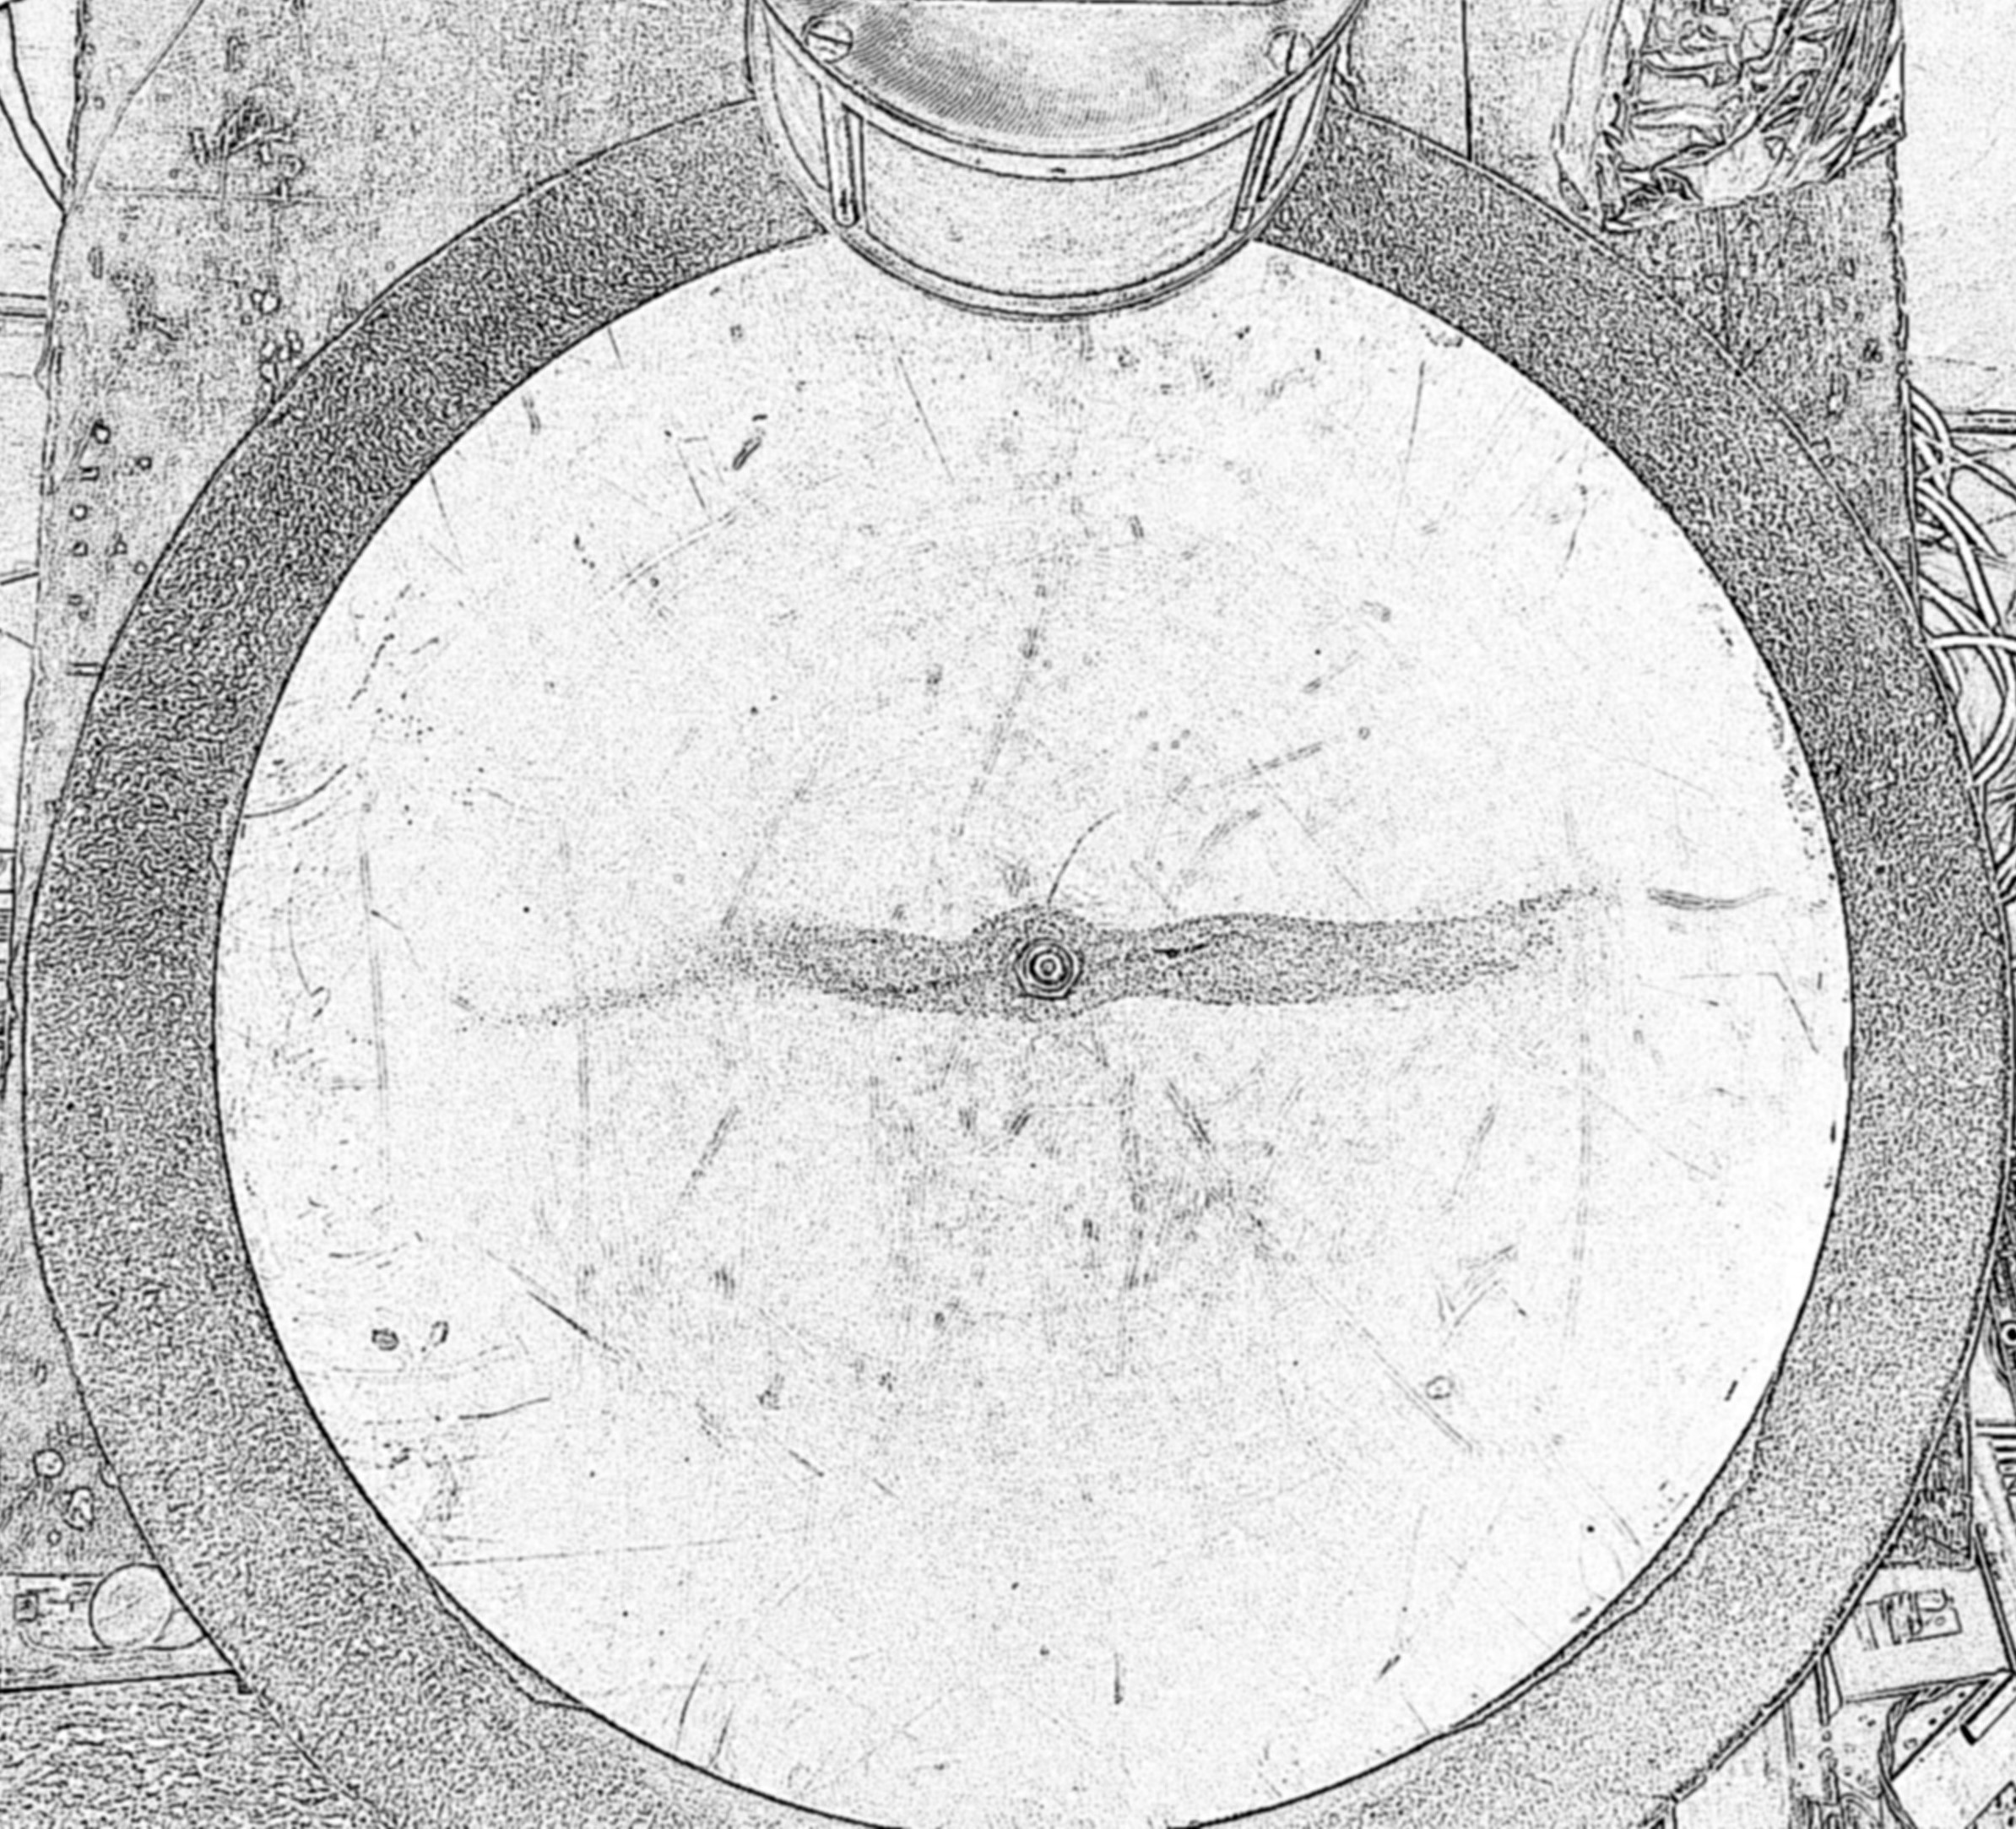
\includegraphics [height = 6cm] {Lab_7_Form_1.jpg} & 26 \\ [21ex]
        \hline
        2 & \center 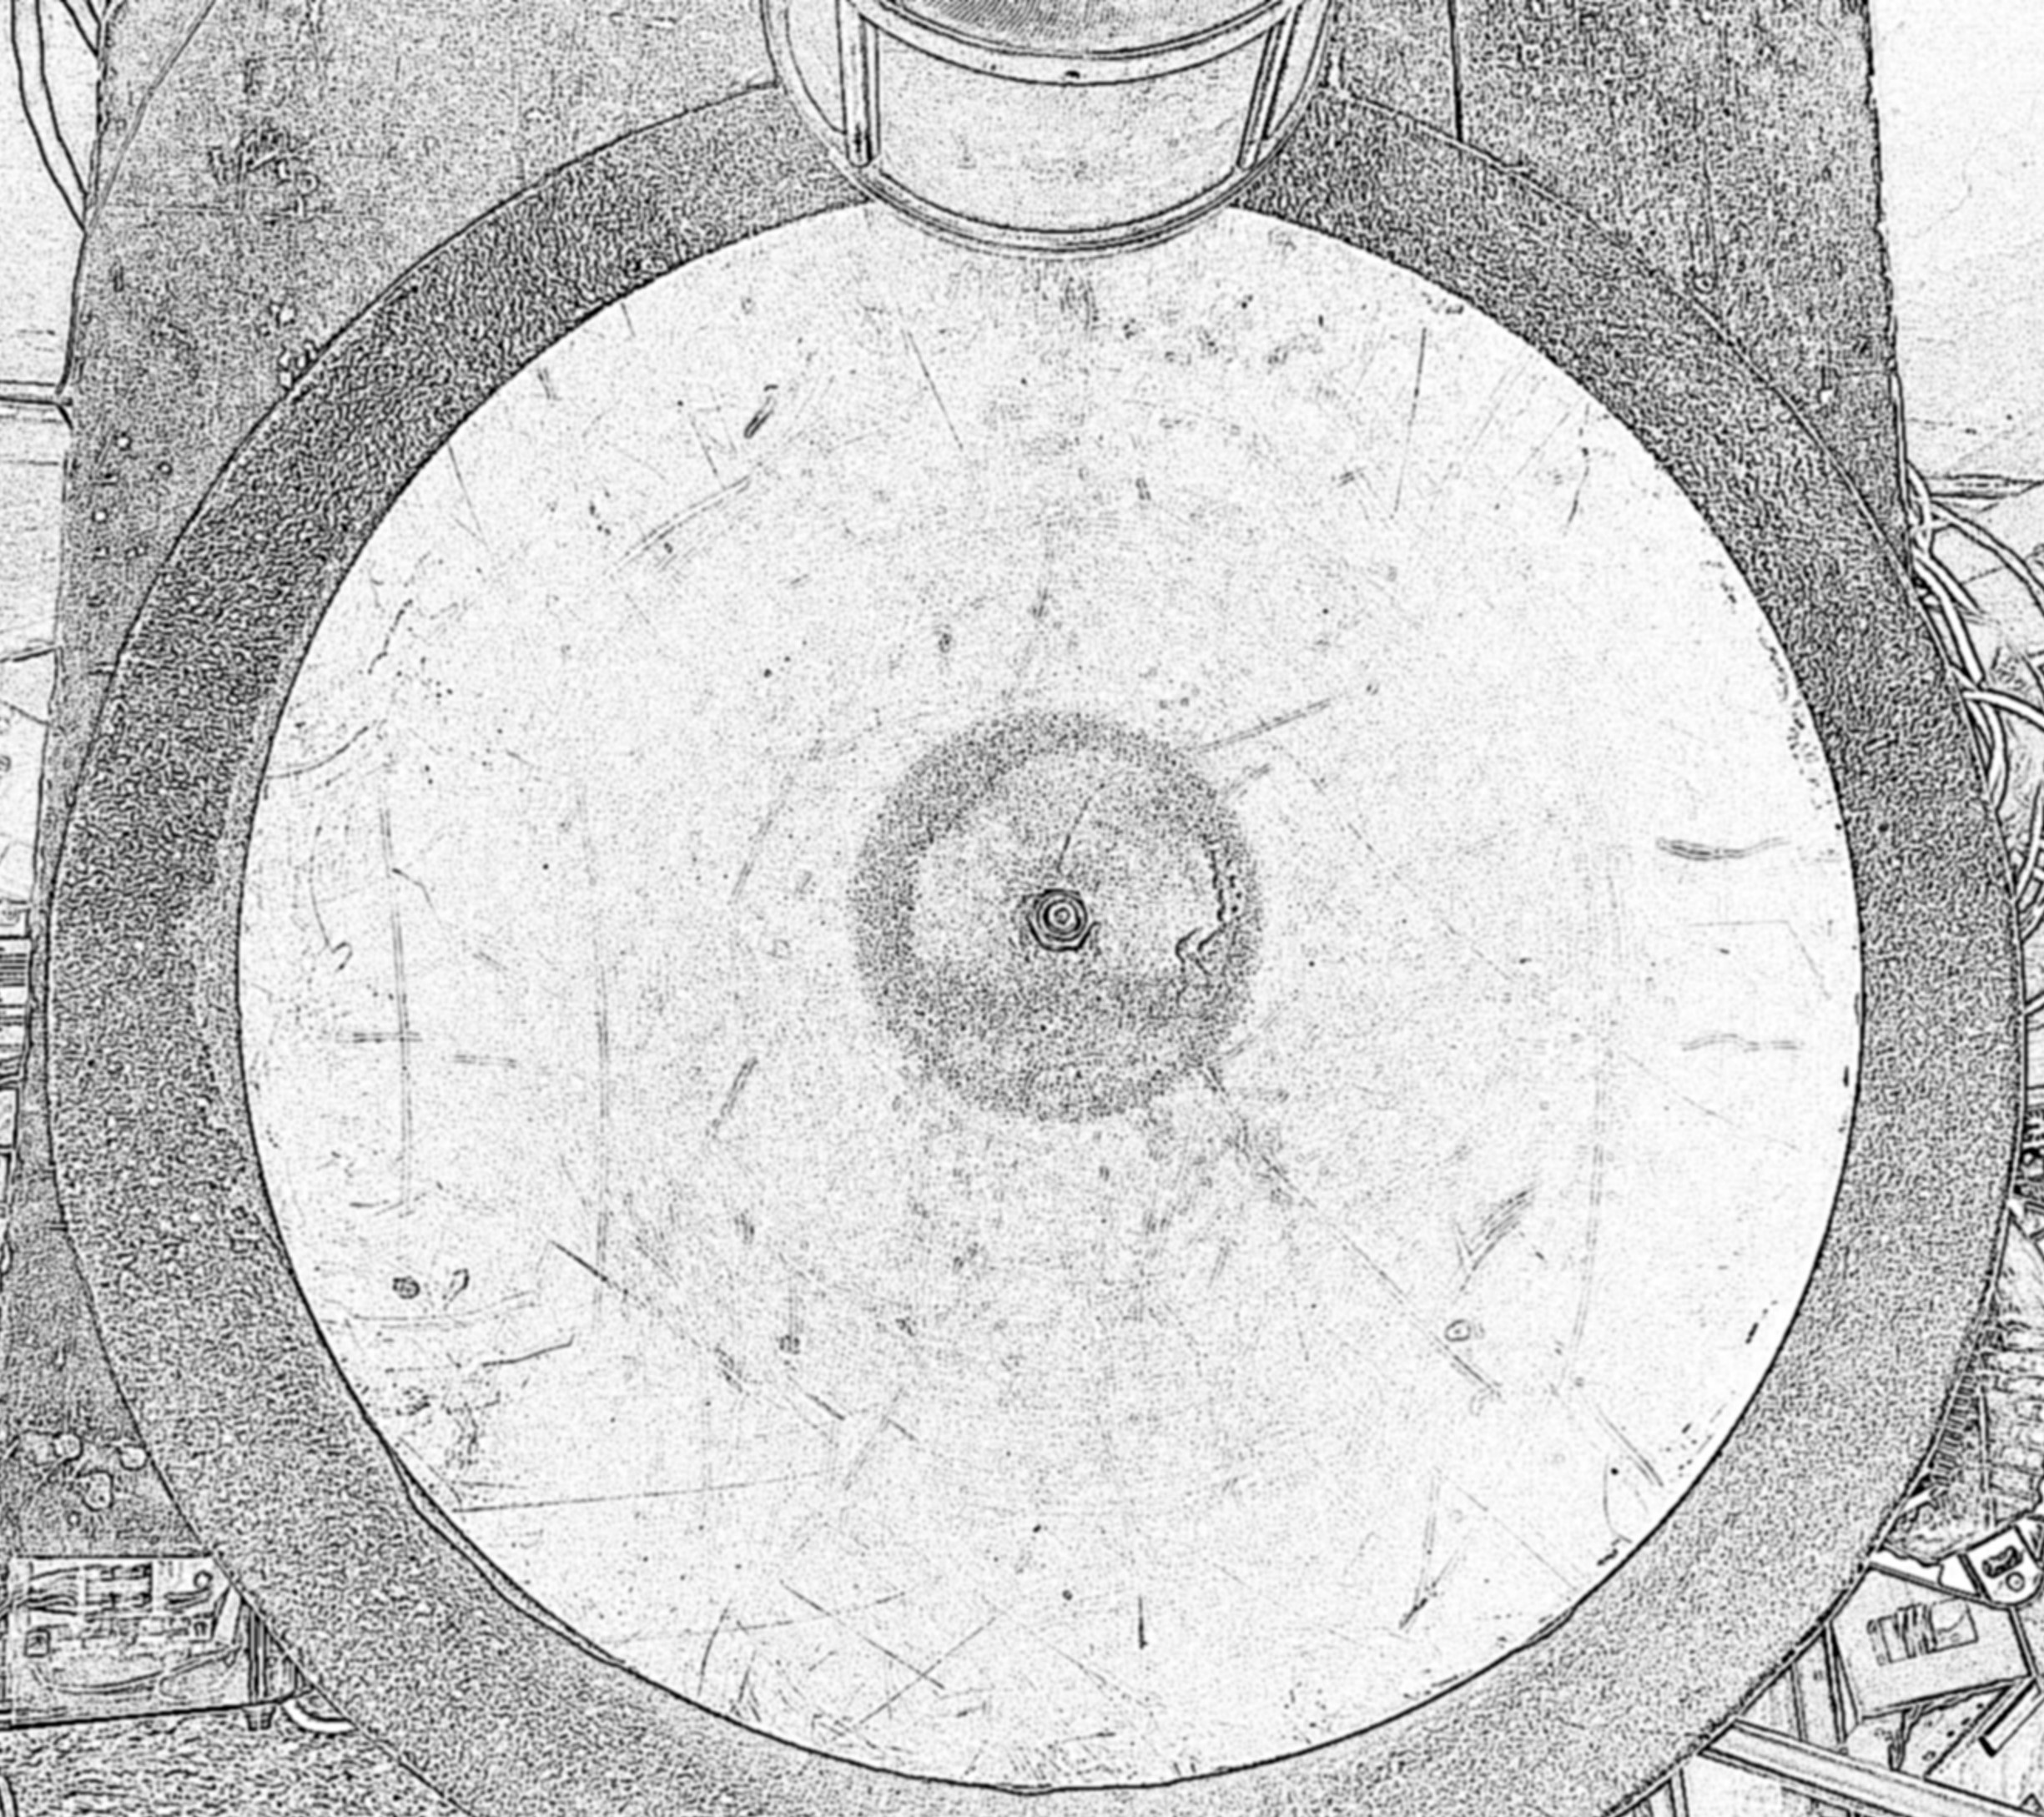
\includegraphics [height = 6cm] {Lab_7_Form_2.jpg} & 46 \\ [21ex]
        \hline
        3 & \center 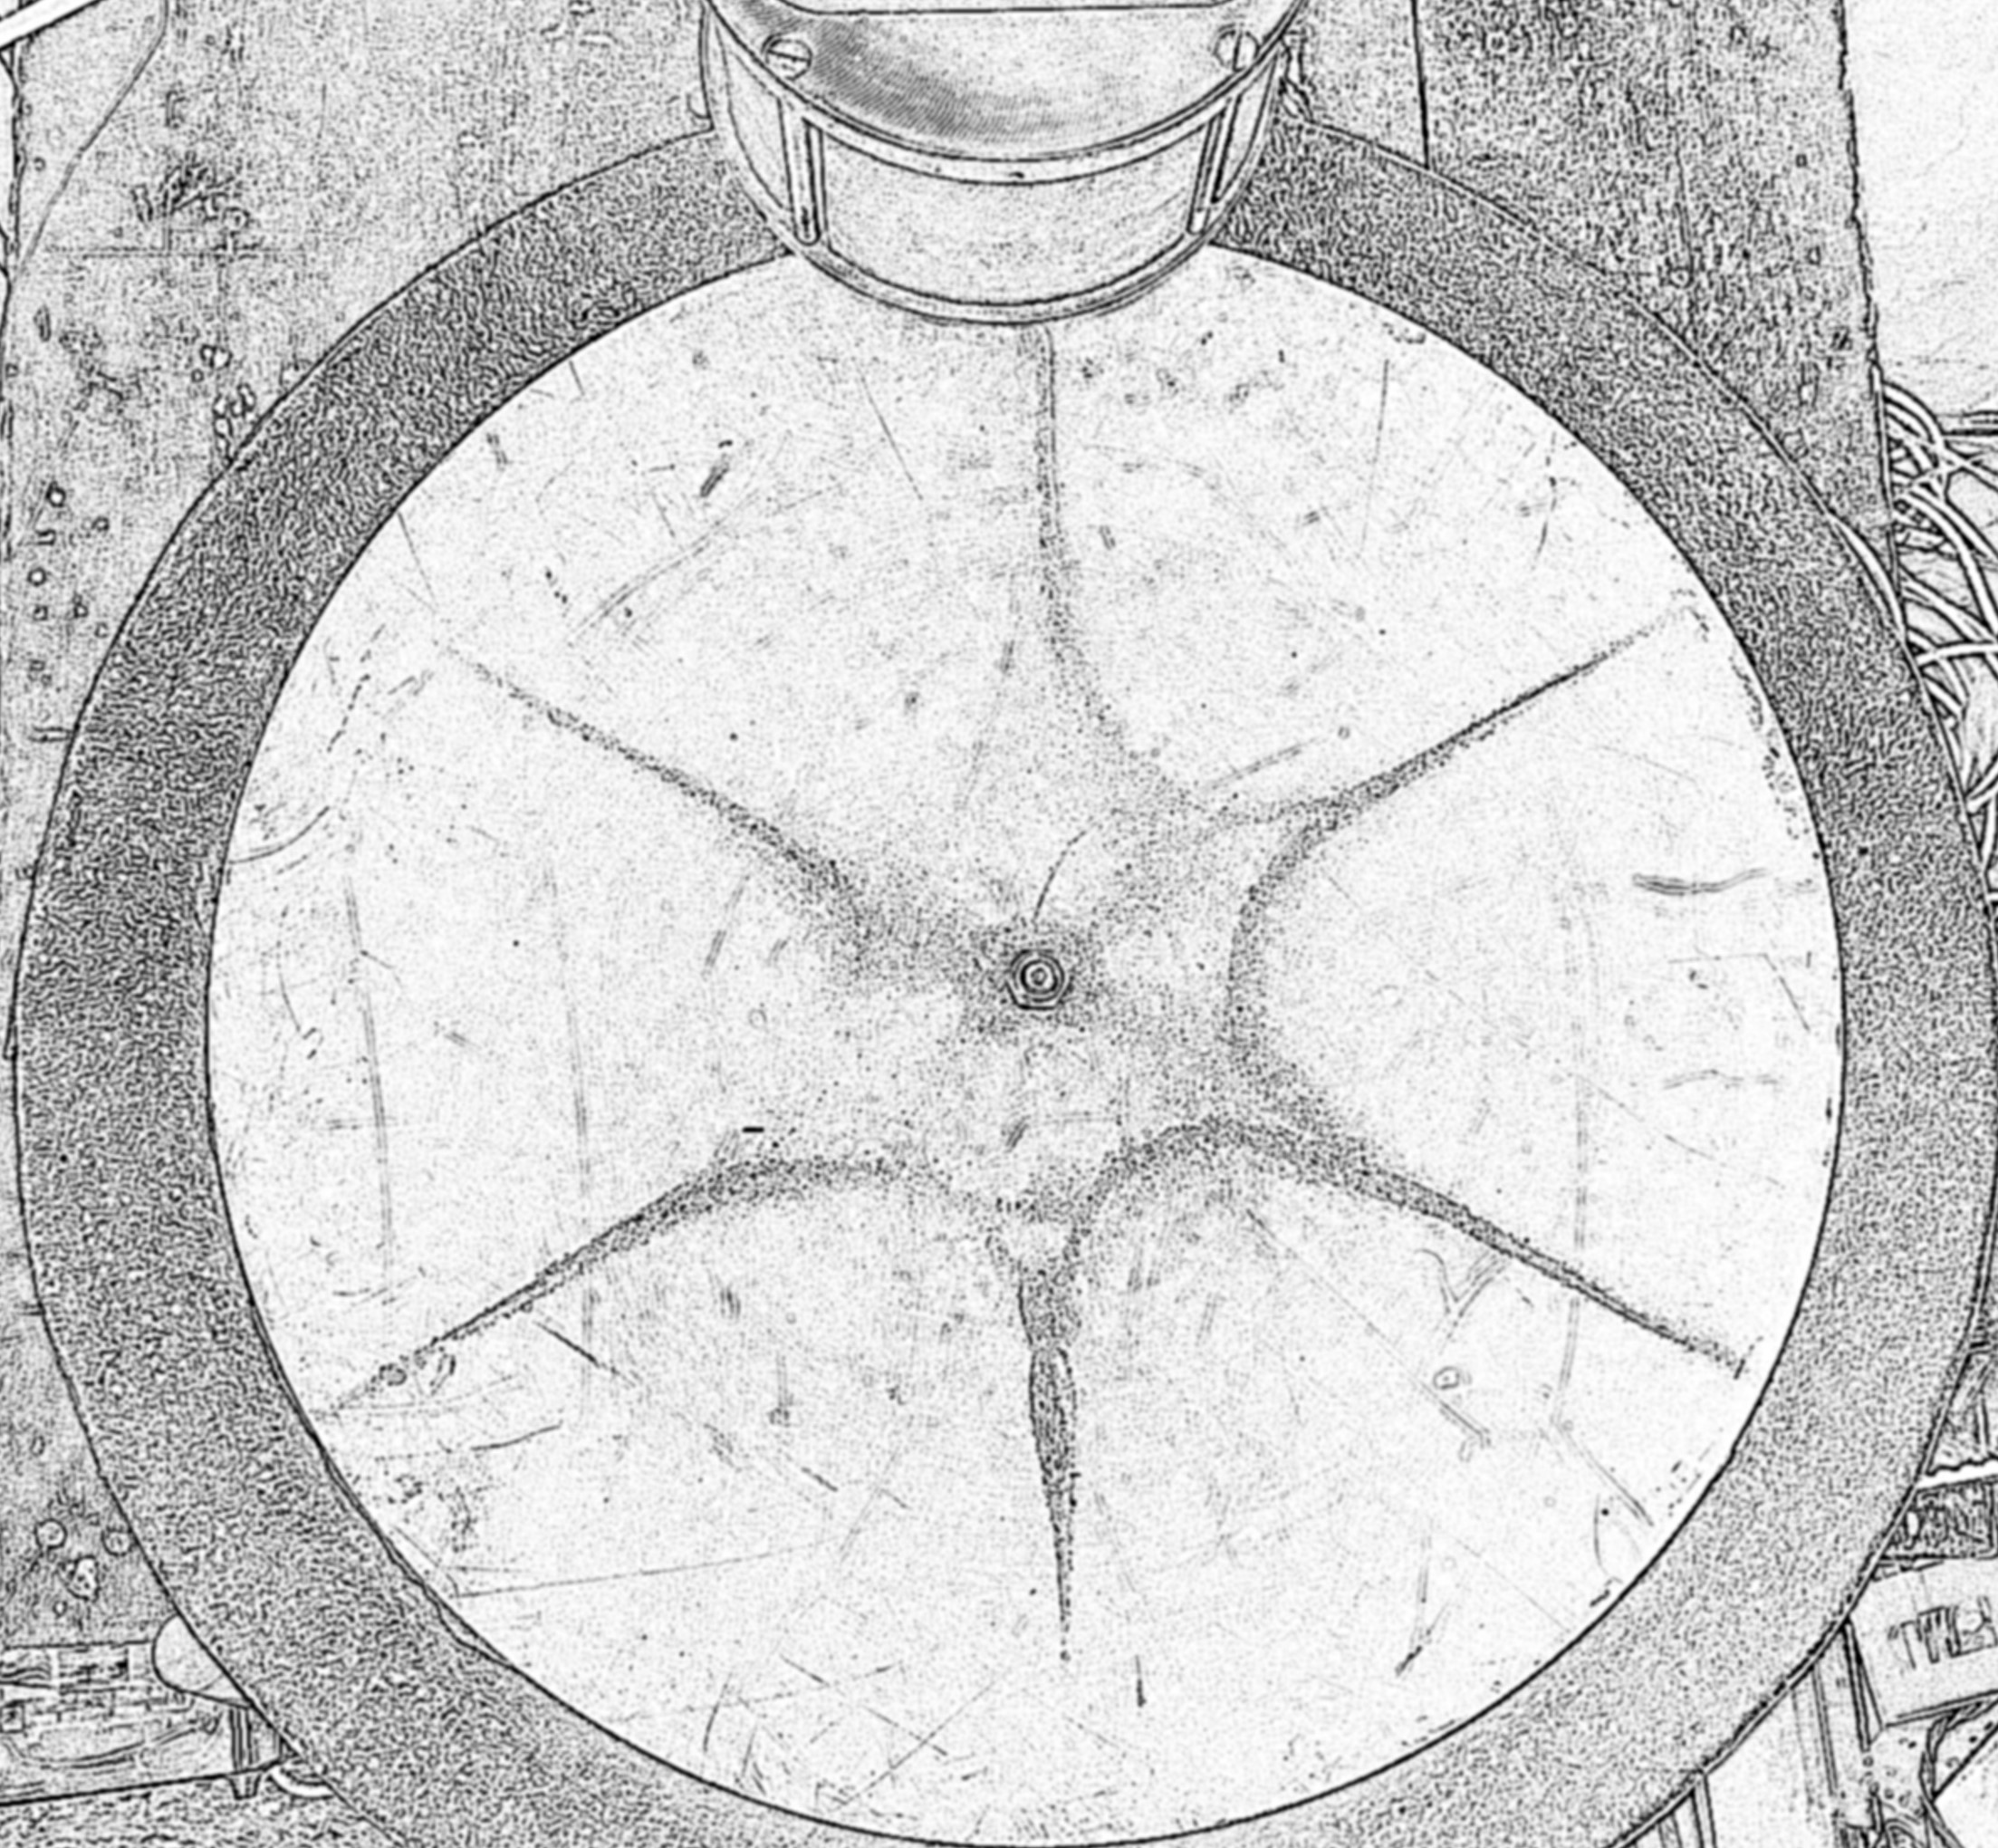
\includegraphics [height = 6cm] {Lab_7_Form_3.jpg} & 150 \\ [21ex]
        \hline
        4 & \center 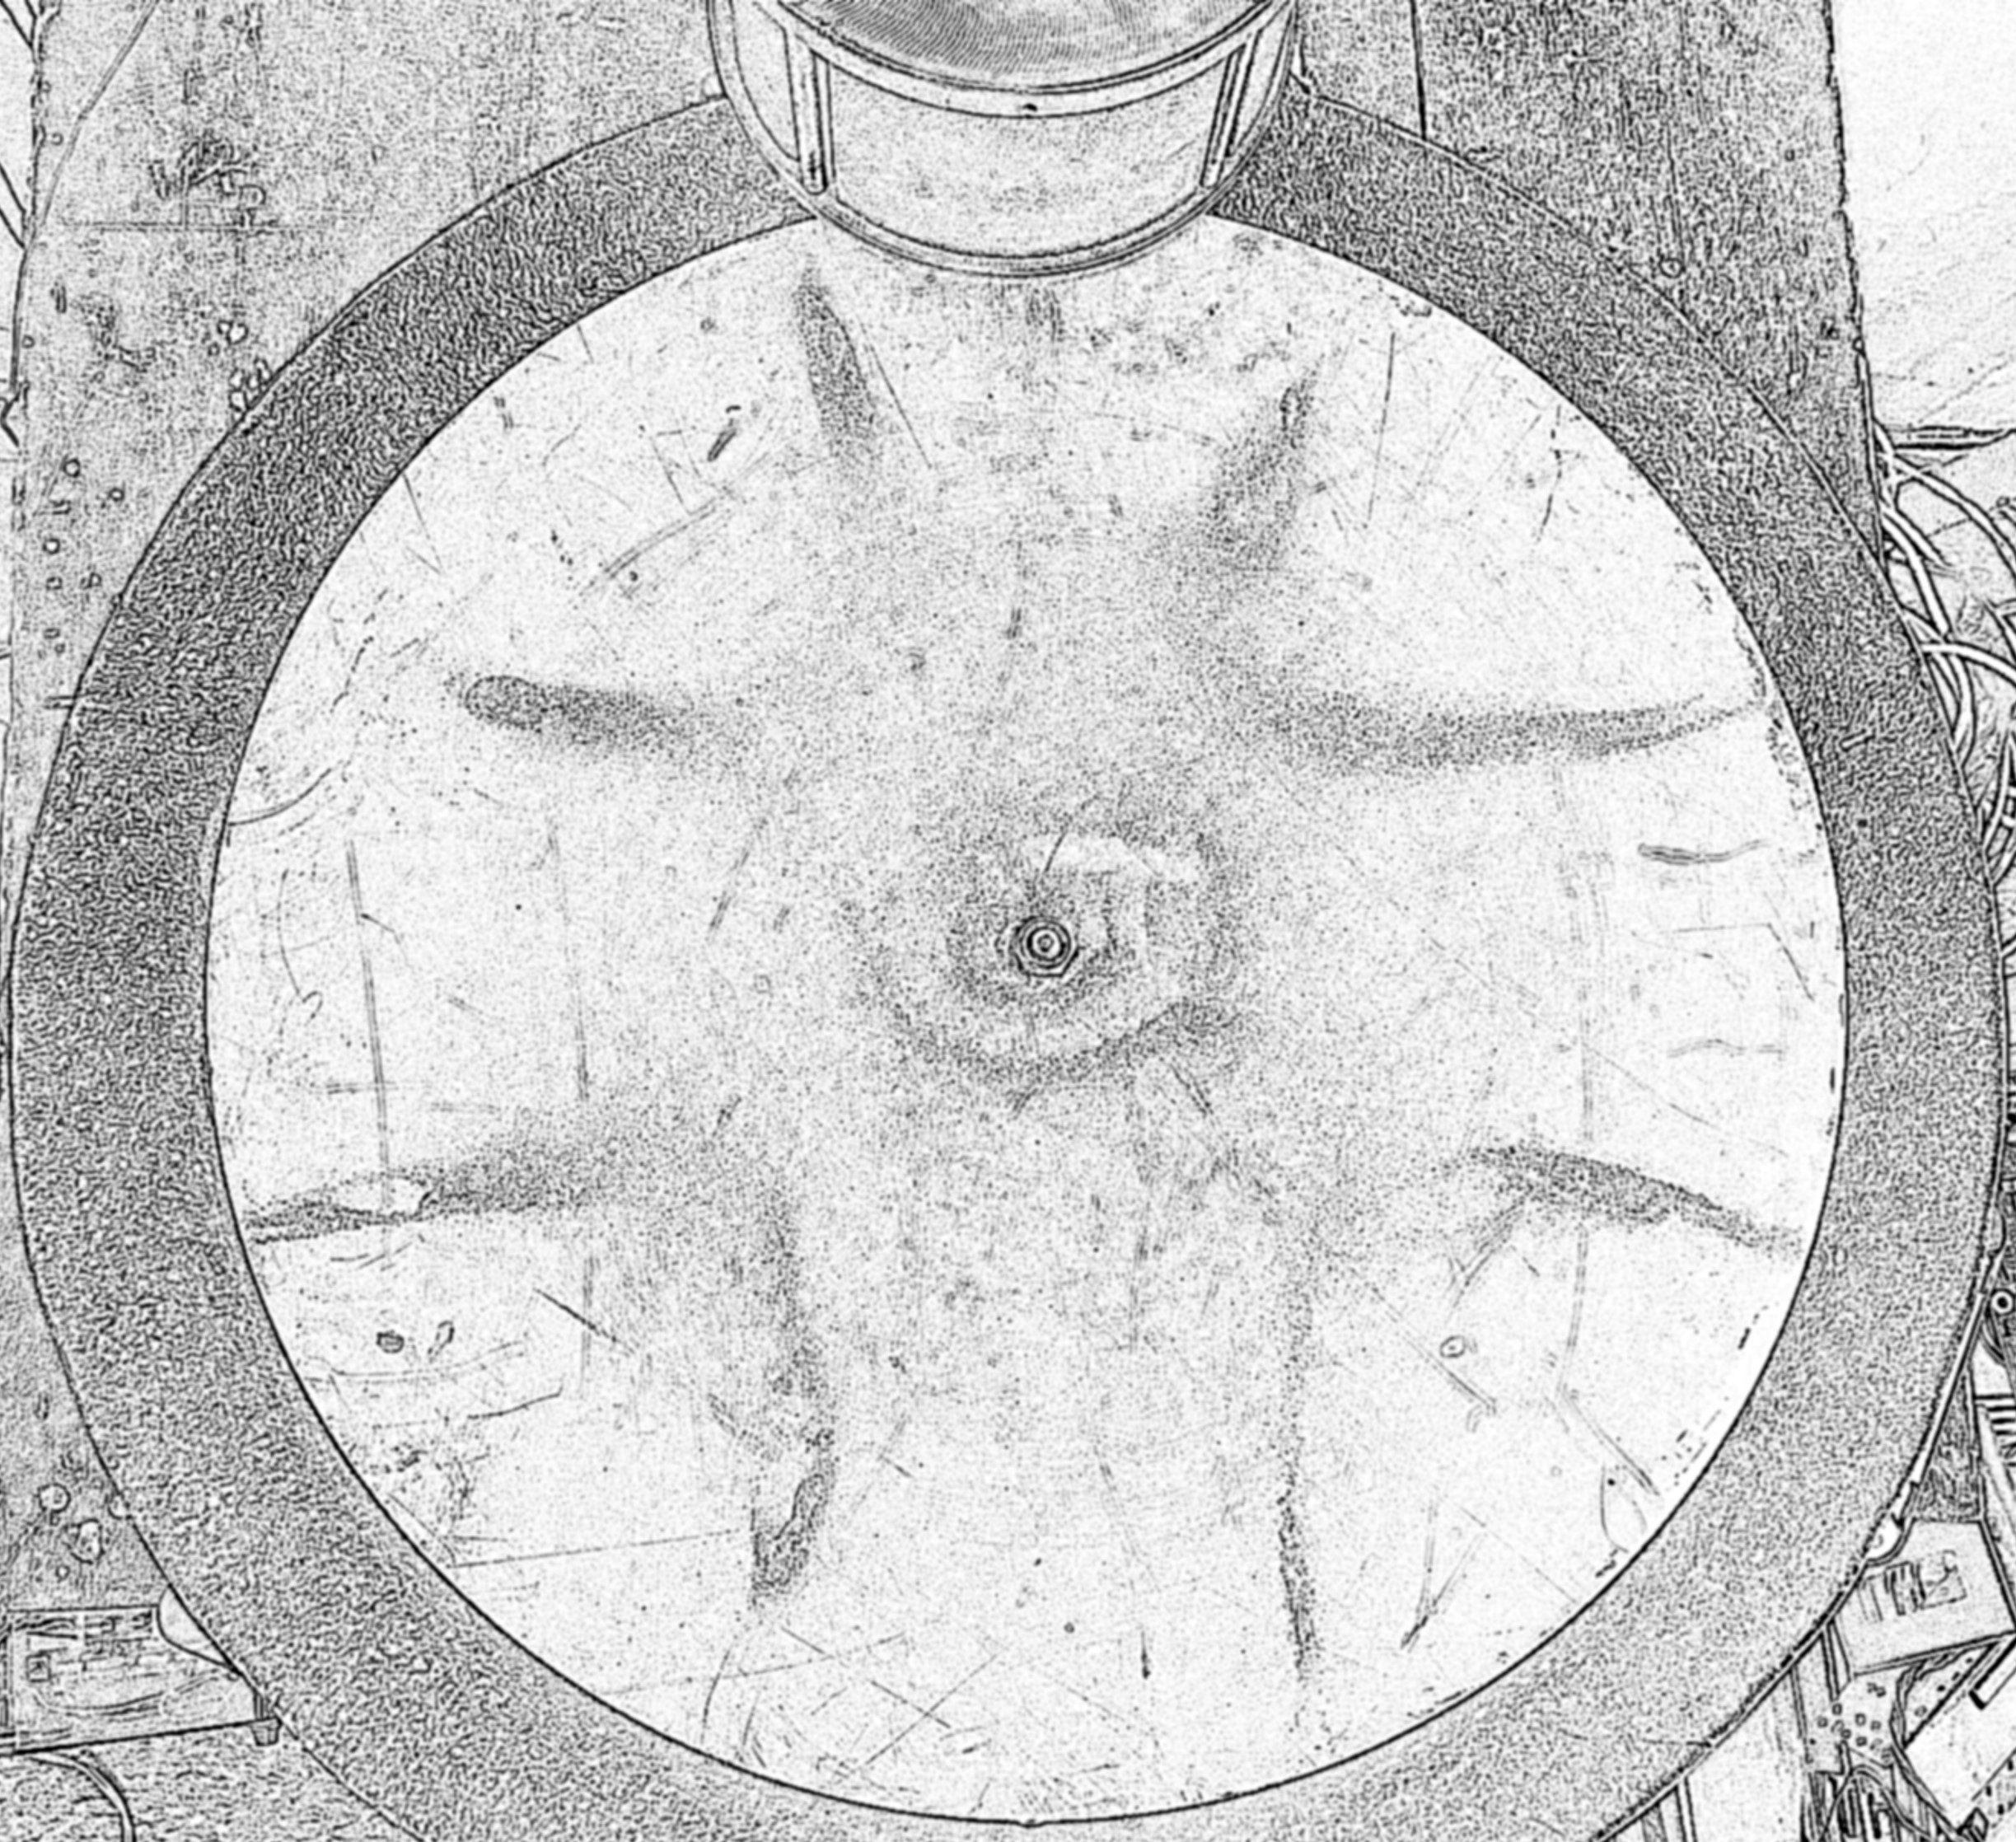
\includegraphics [height = 6cm] {Lab_7_Form_4.jpg} & 260 \\ [21ex]
        \hline
        5 & \center 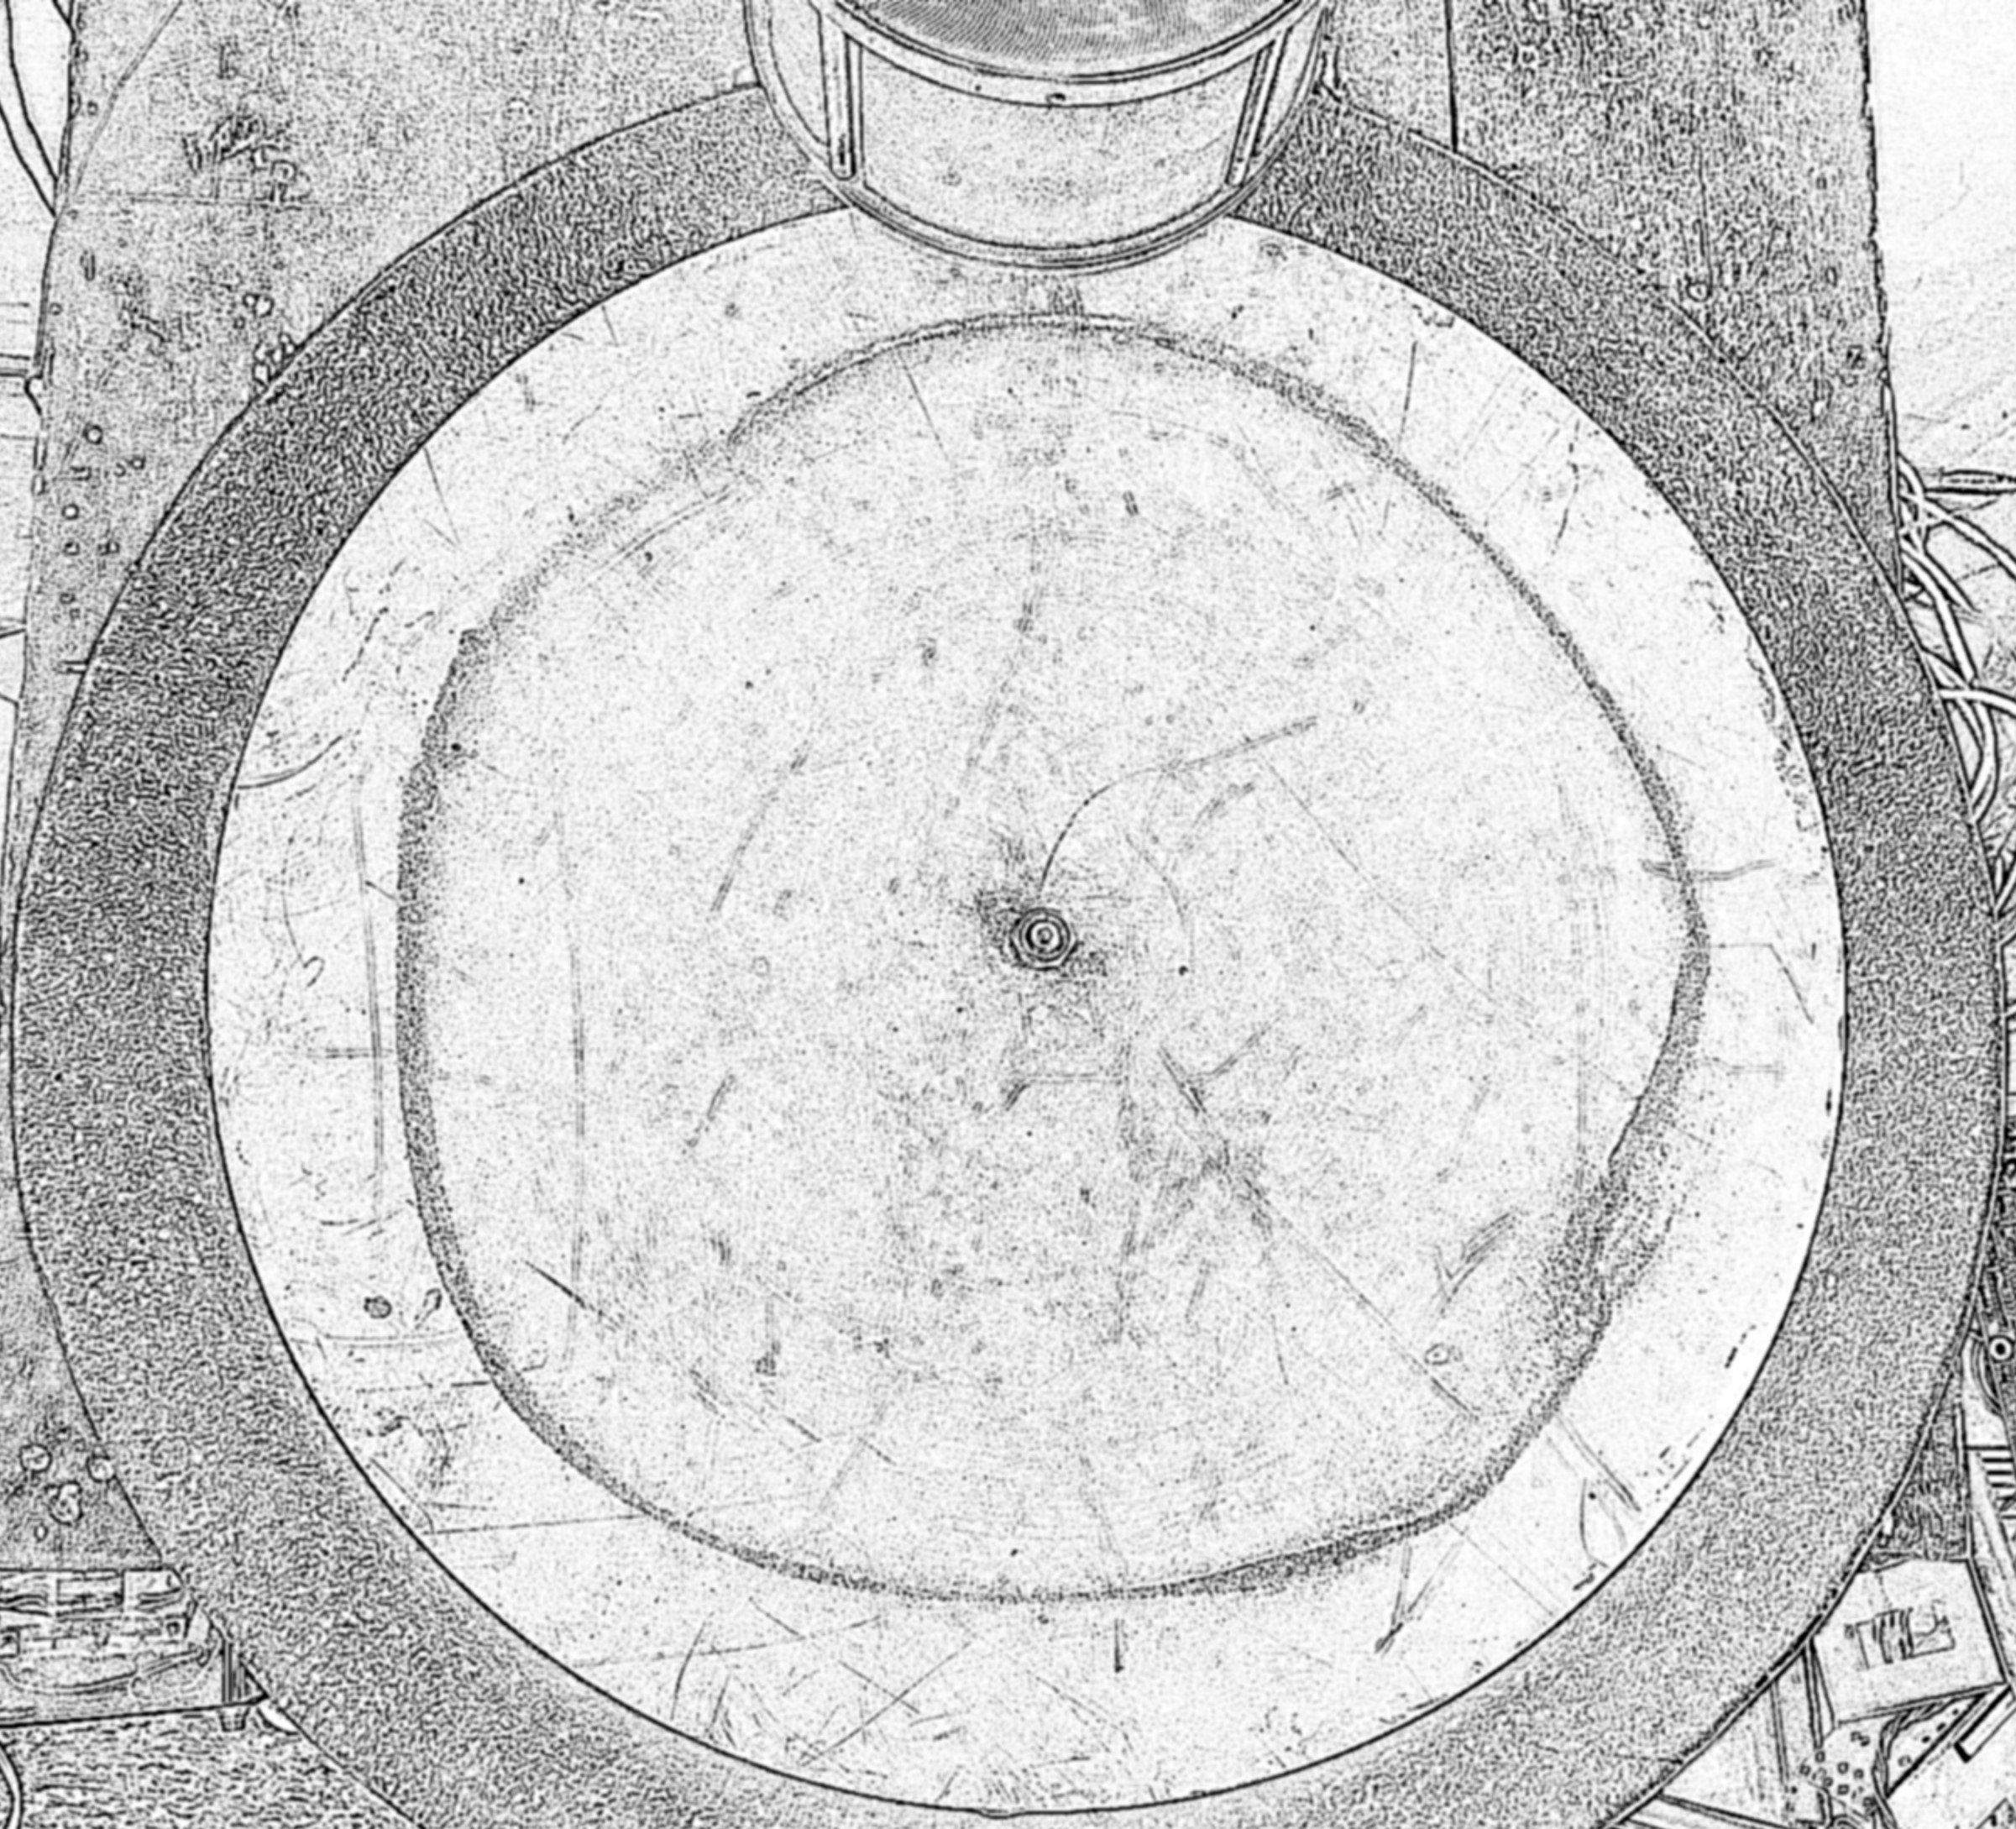
\includegraphics [height = 6cm] {Lab_7_Form_5.jpg} & 285 \\ [21ex]
        \hline
        6 & \center 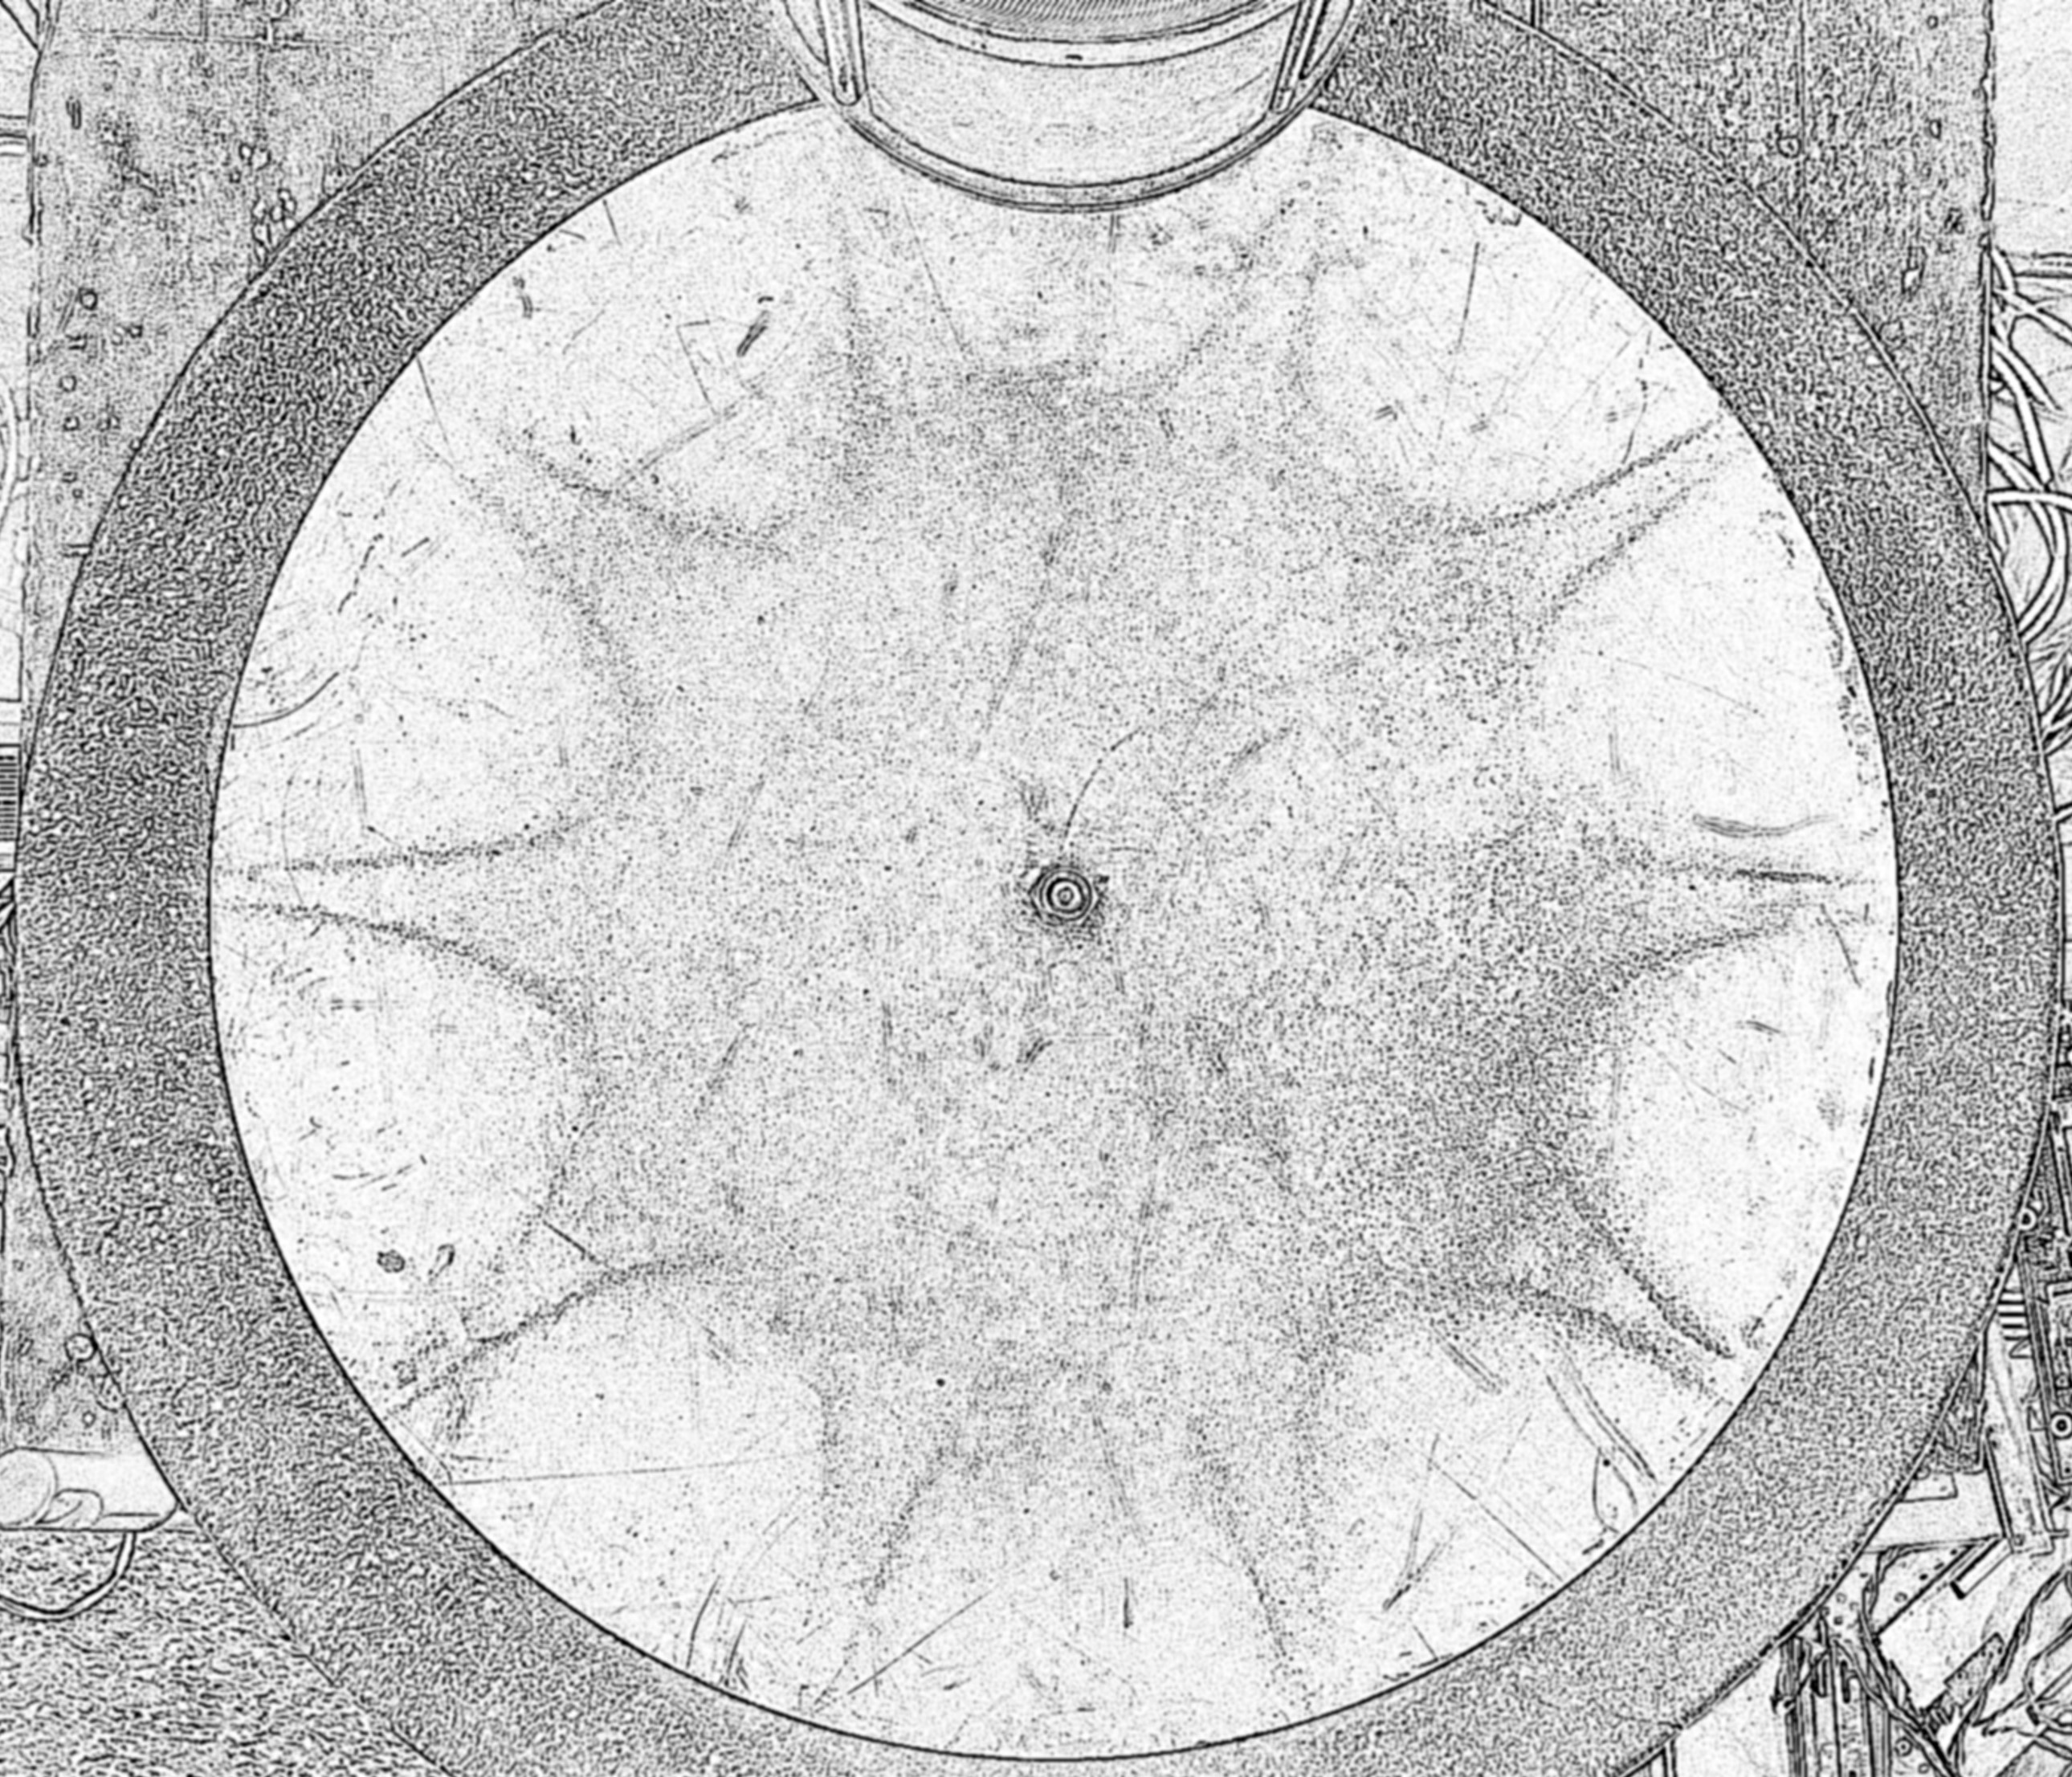
\includegraphics [height = 6cm] {Lab_7_Form_6.jpg} & 405 \\ [21ex]
        \hline
        7 & \center 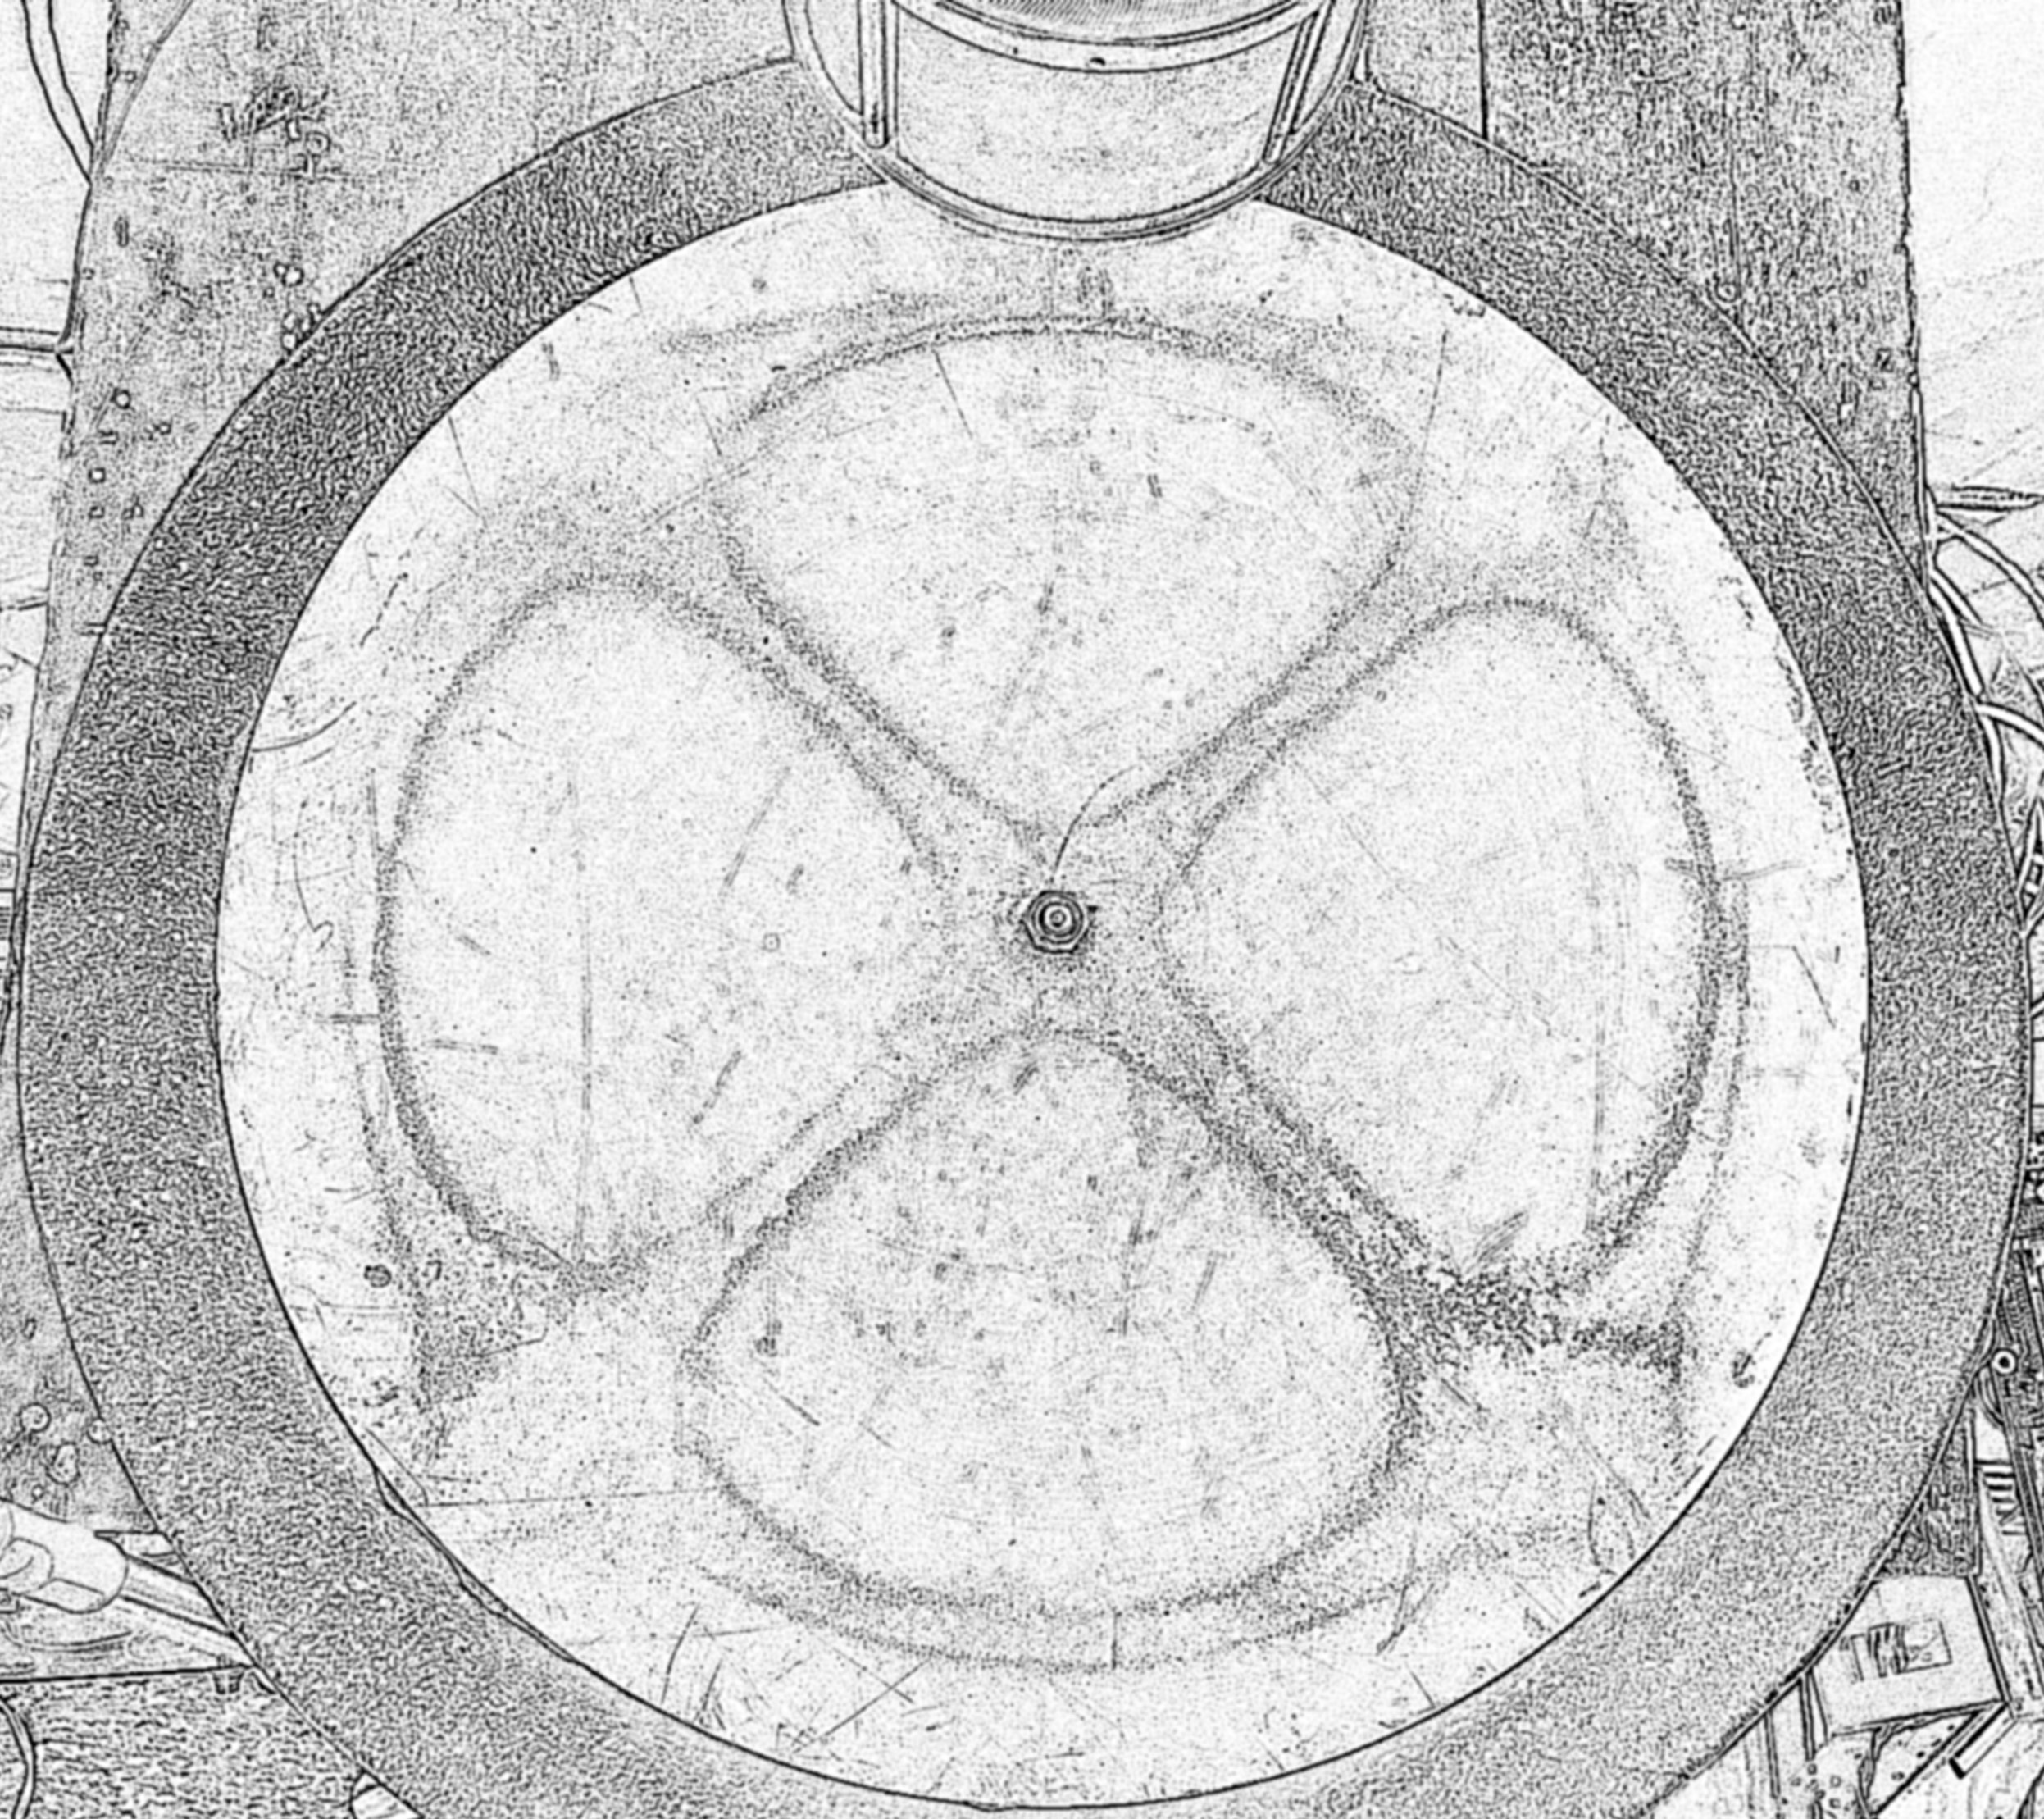
\includegraphics [height = 6cm] {Lab_7_Form_7.jpg} & 435 \\ [21ex]
        \hline
        8 & \center 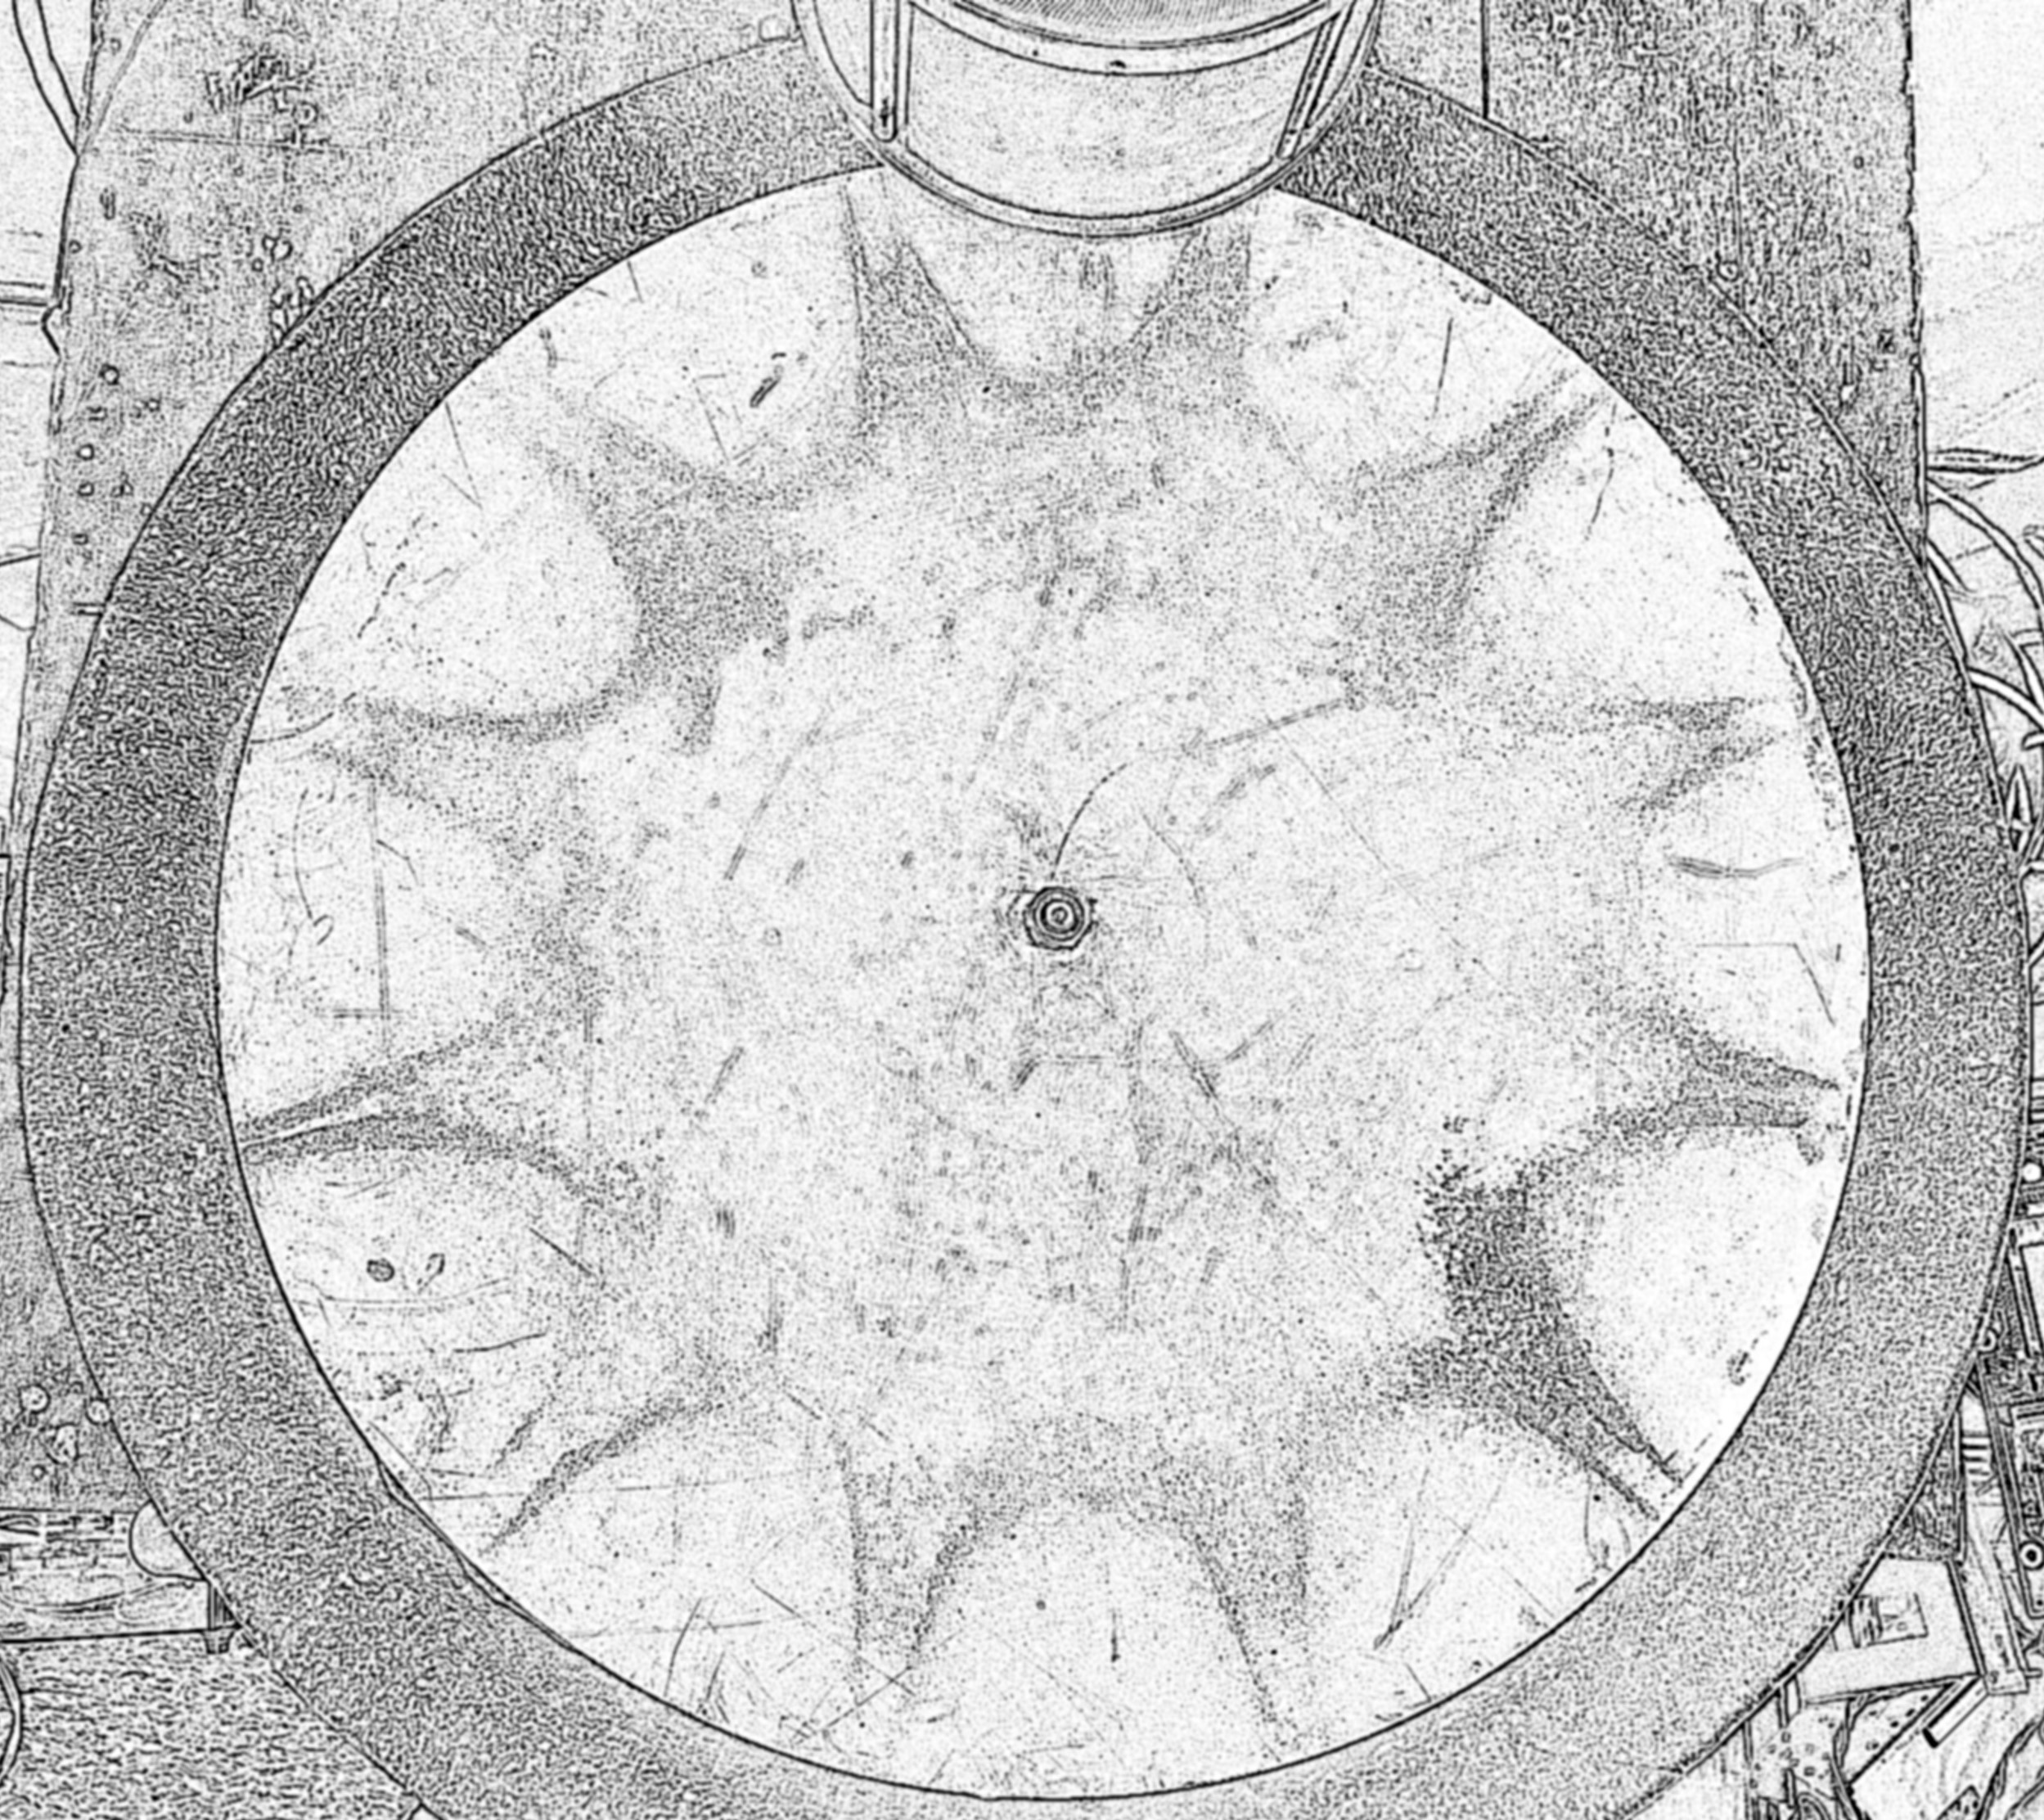
\includegraphics [height = 6cm] {Lab_7_Form_8.jpg} & 562 \\ [21ex]
        \hline
        9 & \center 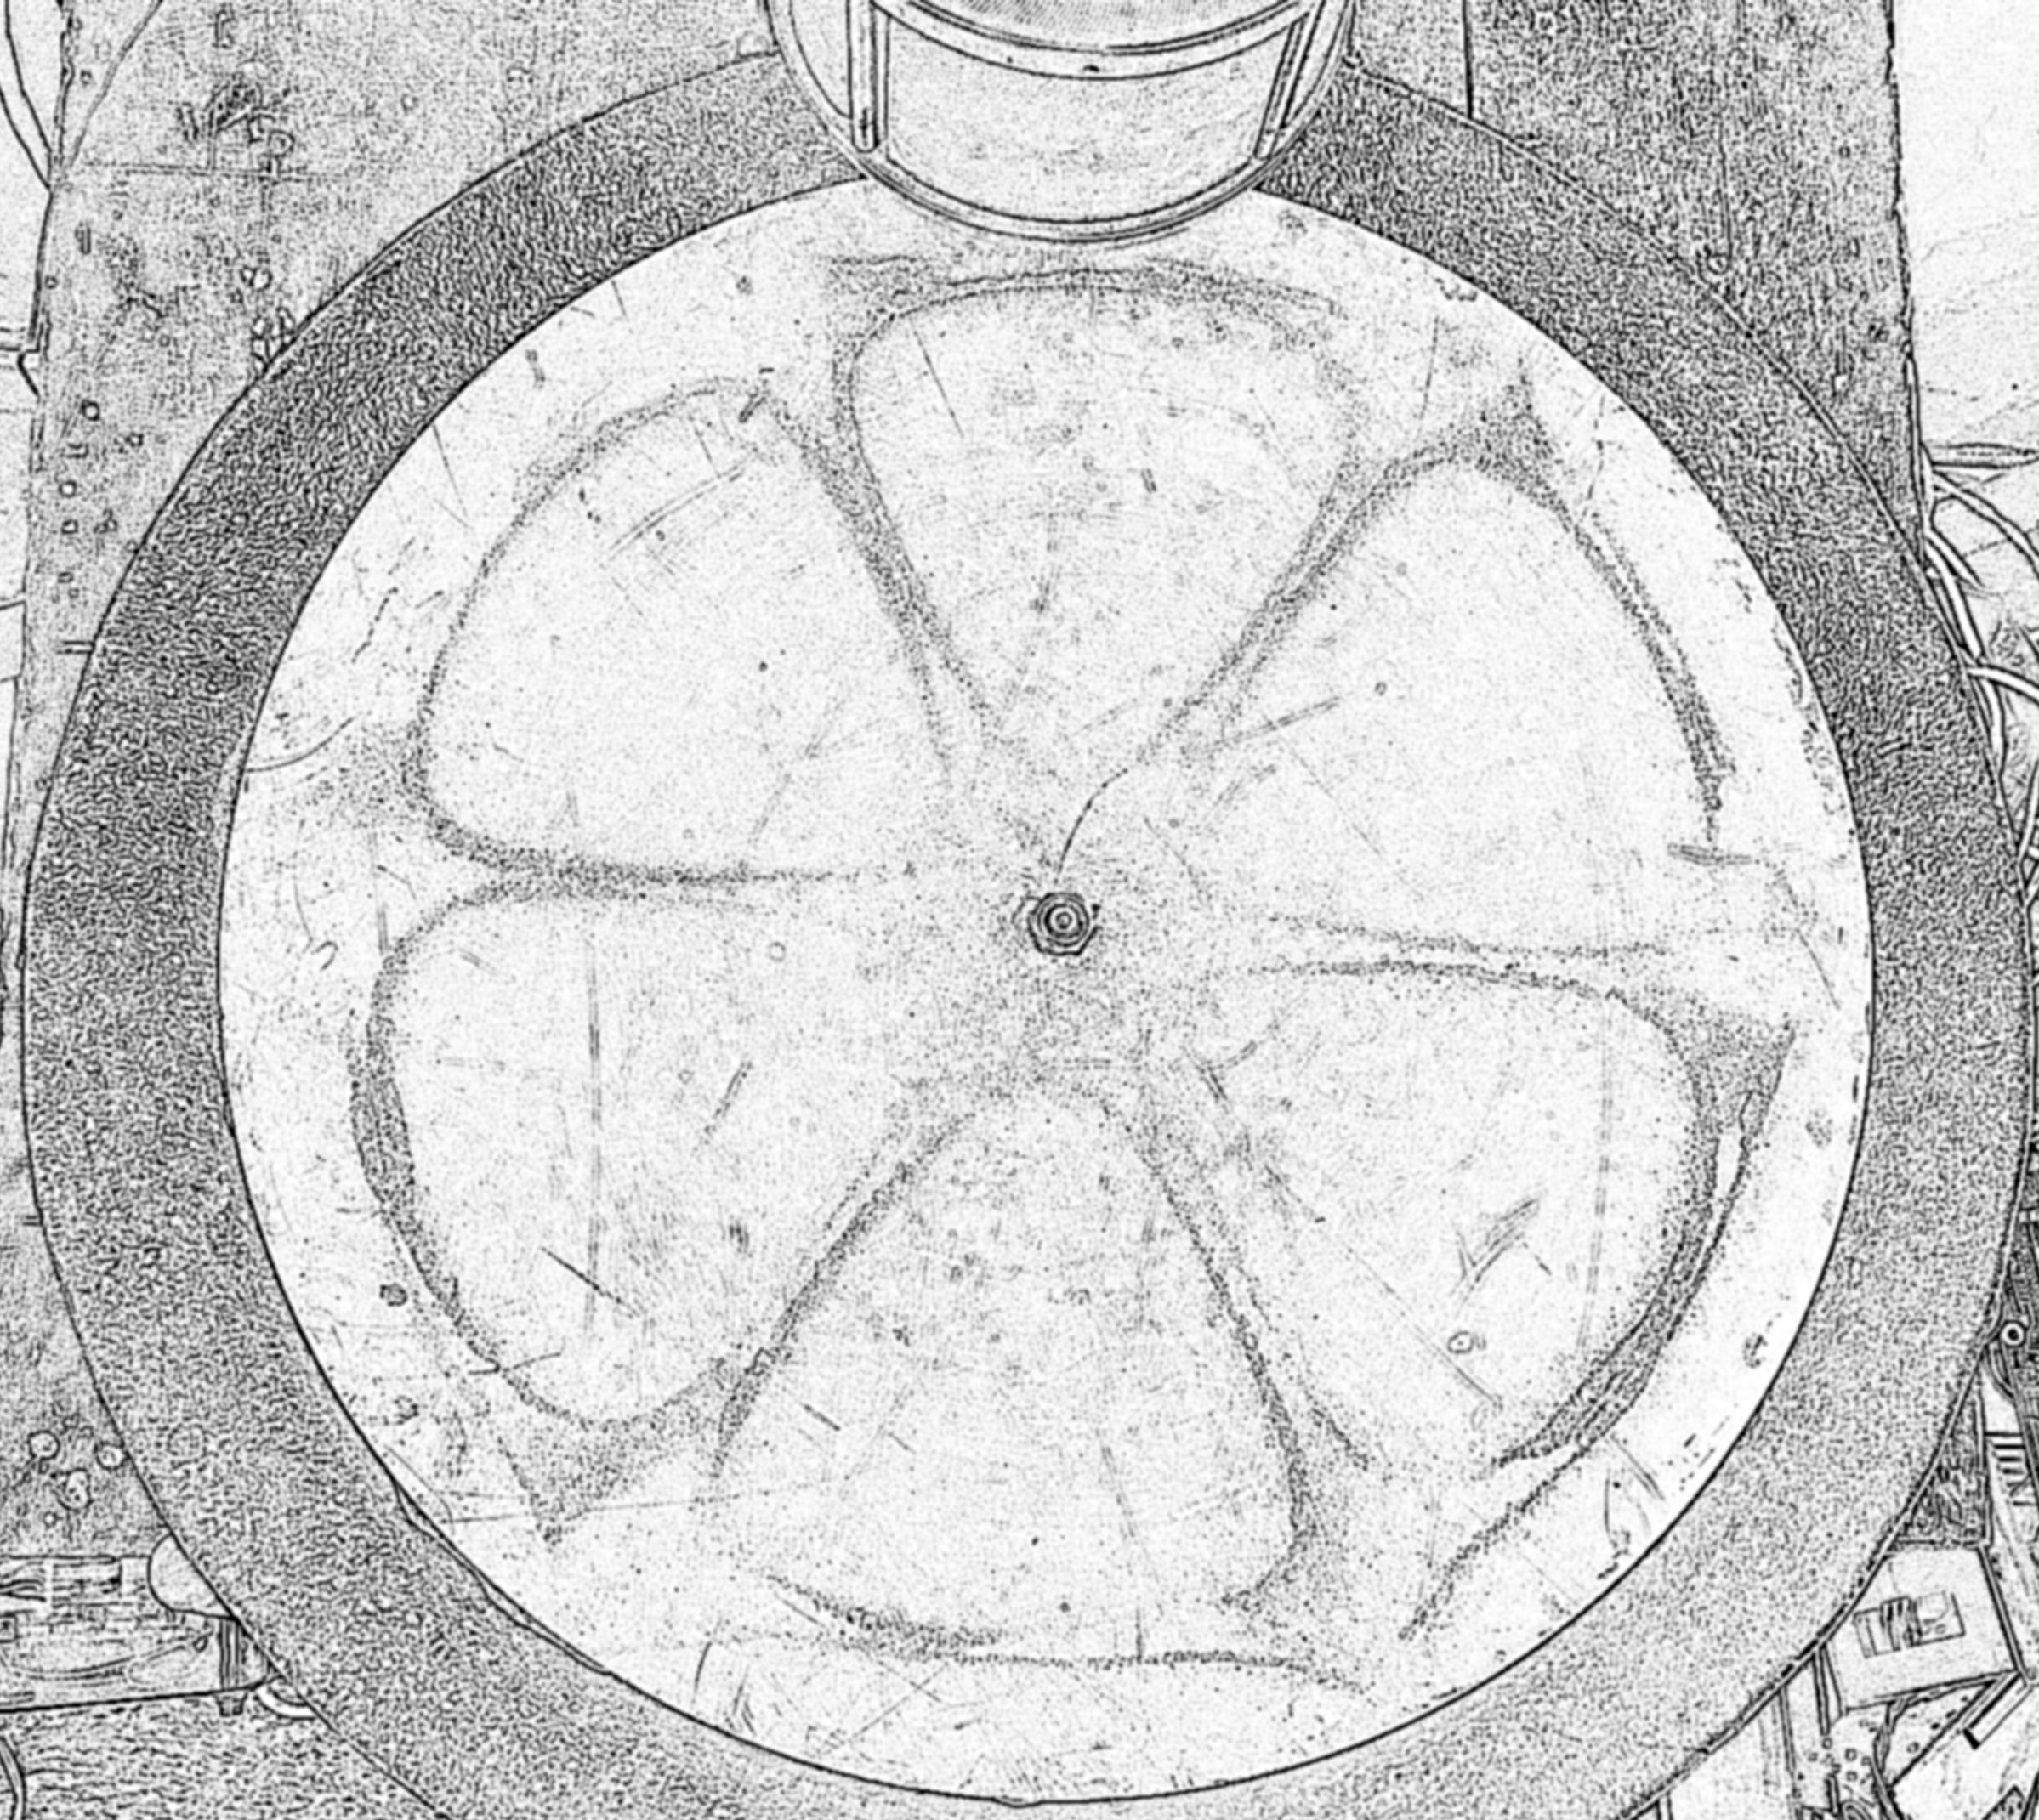
\includegraphics [height = 6cm] {Lab_7_Form_9.jpg} & 640 \\ [21ex]
        \hline
        10 & \center 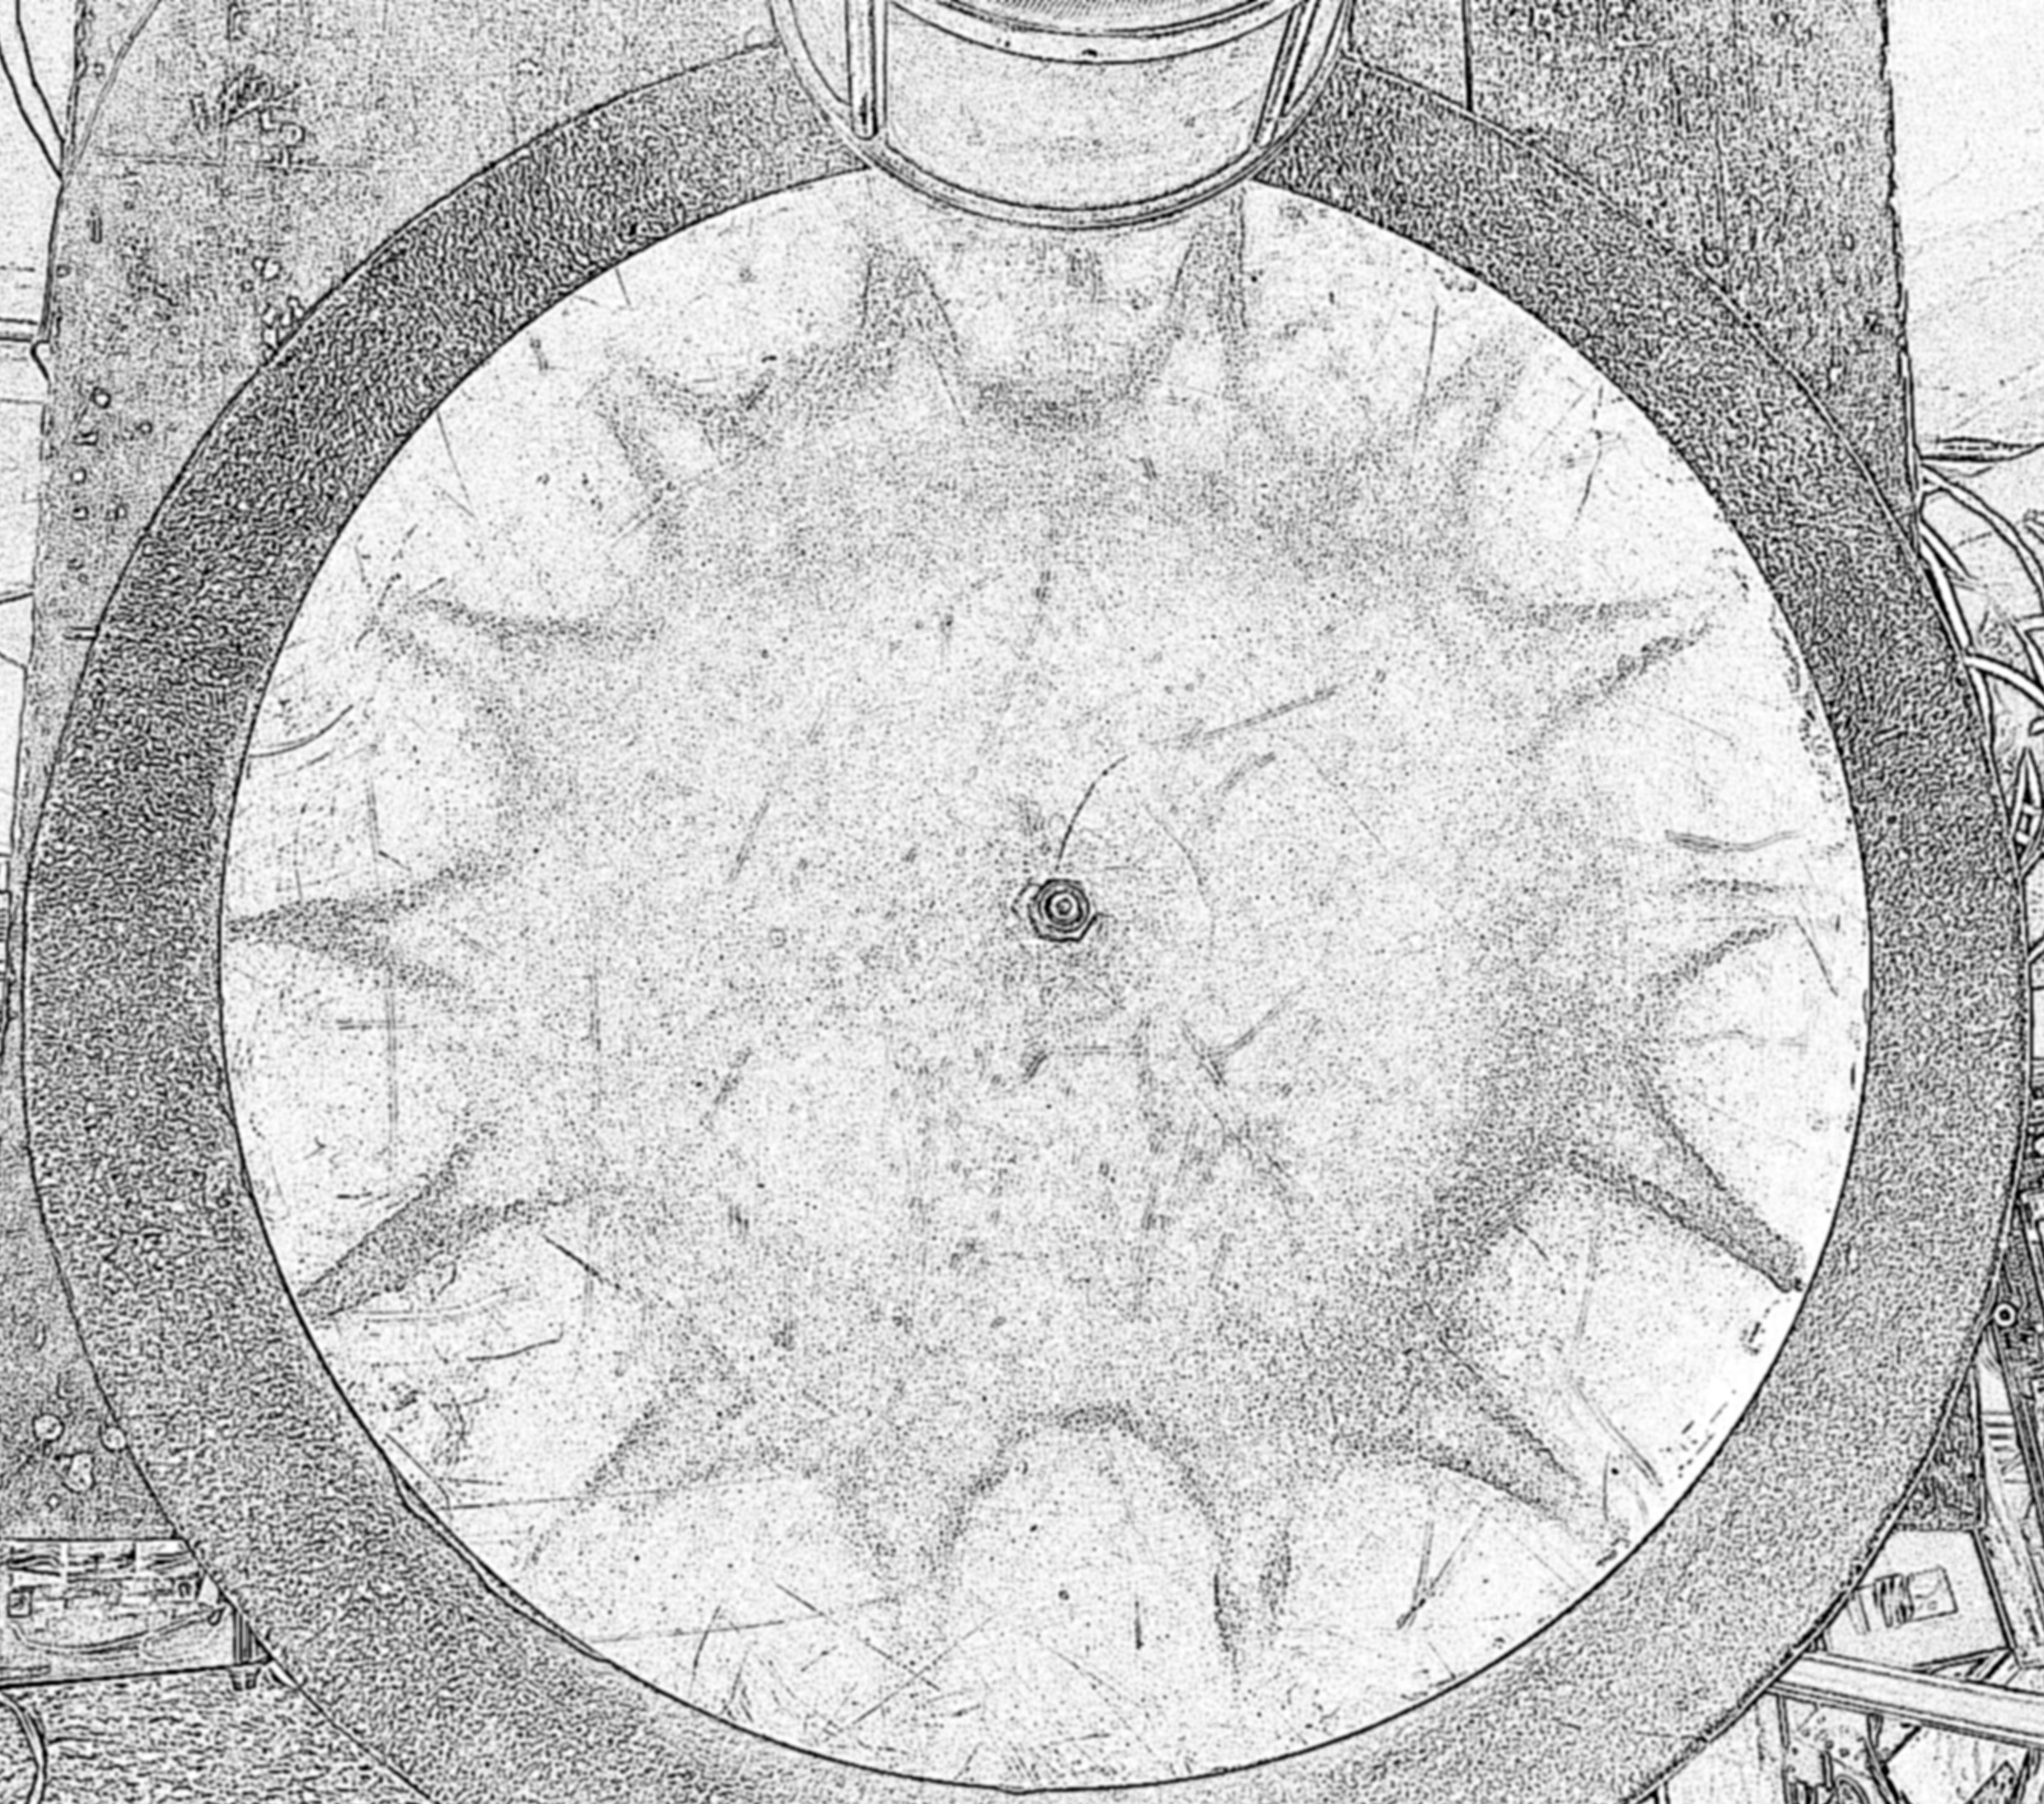
\includegraphics [height = 6cm] {Lab_7_Form_10.jpg} & 760 \\ [21ex]
        \hline
        11 & \center 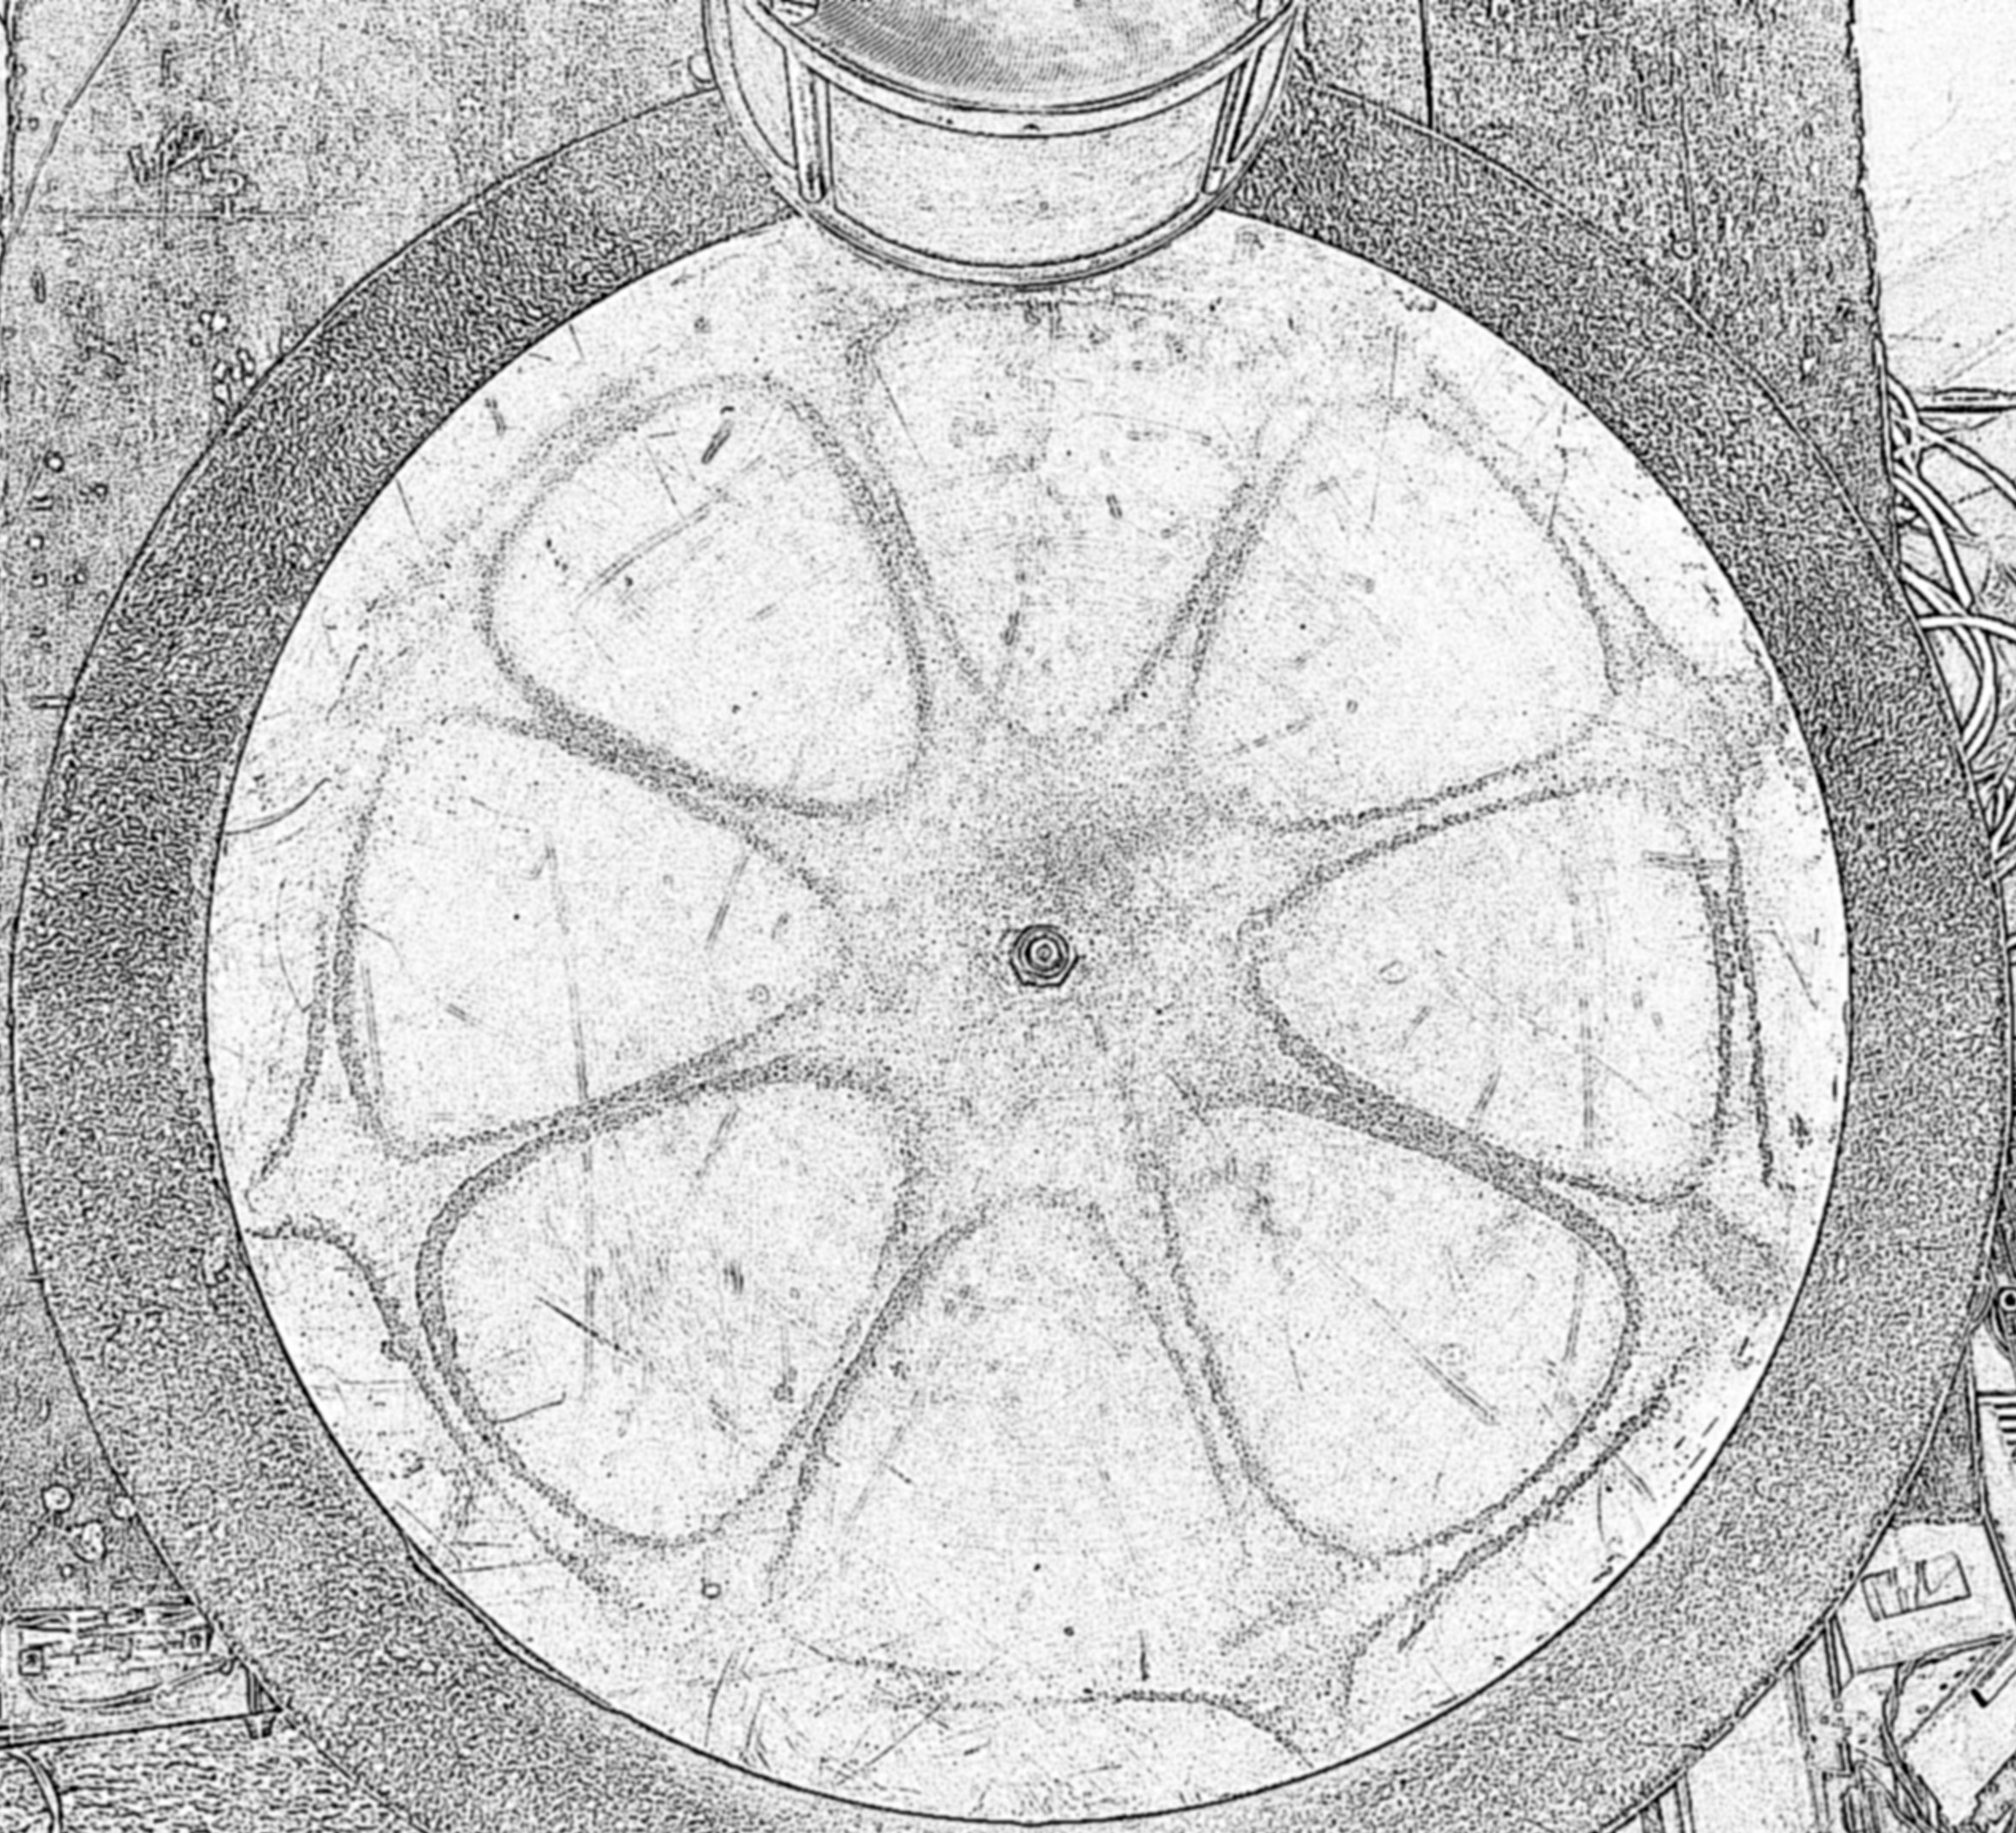
\includegraphics [height = 6cm] {Lab_7_Form_11.jpg} & 890 \\ [21ex]
        \hline
        12 & \center 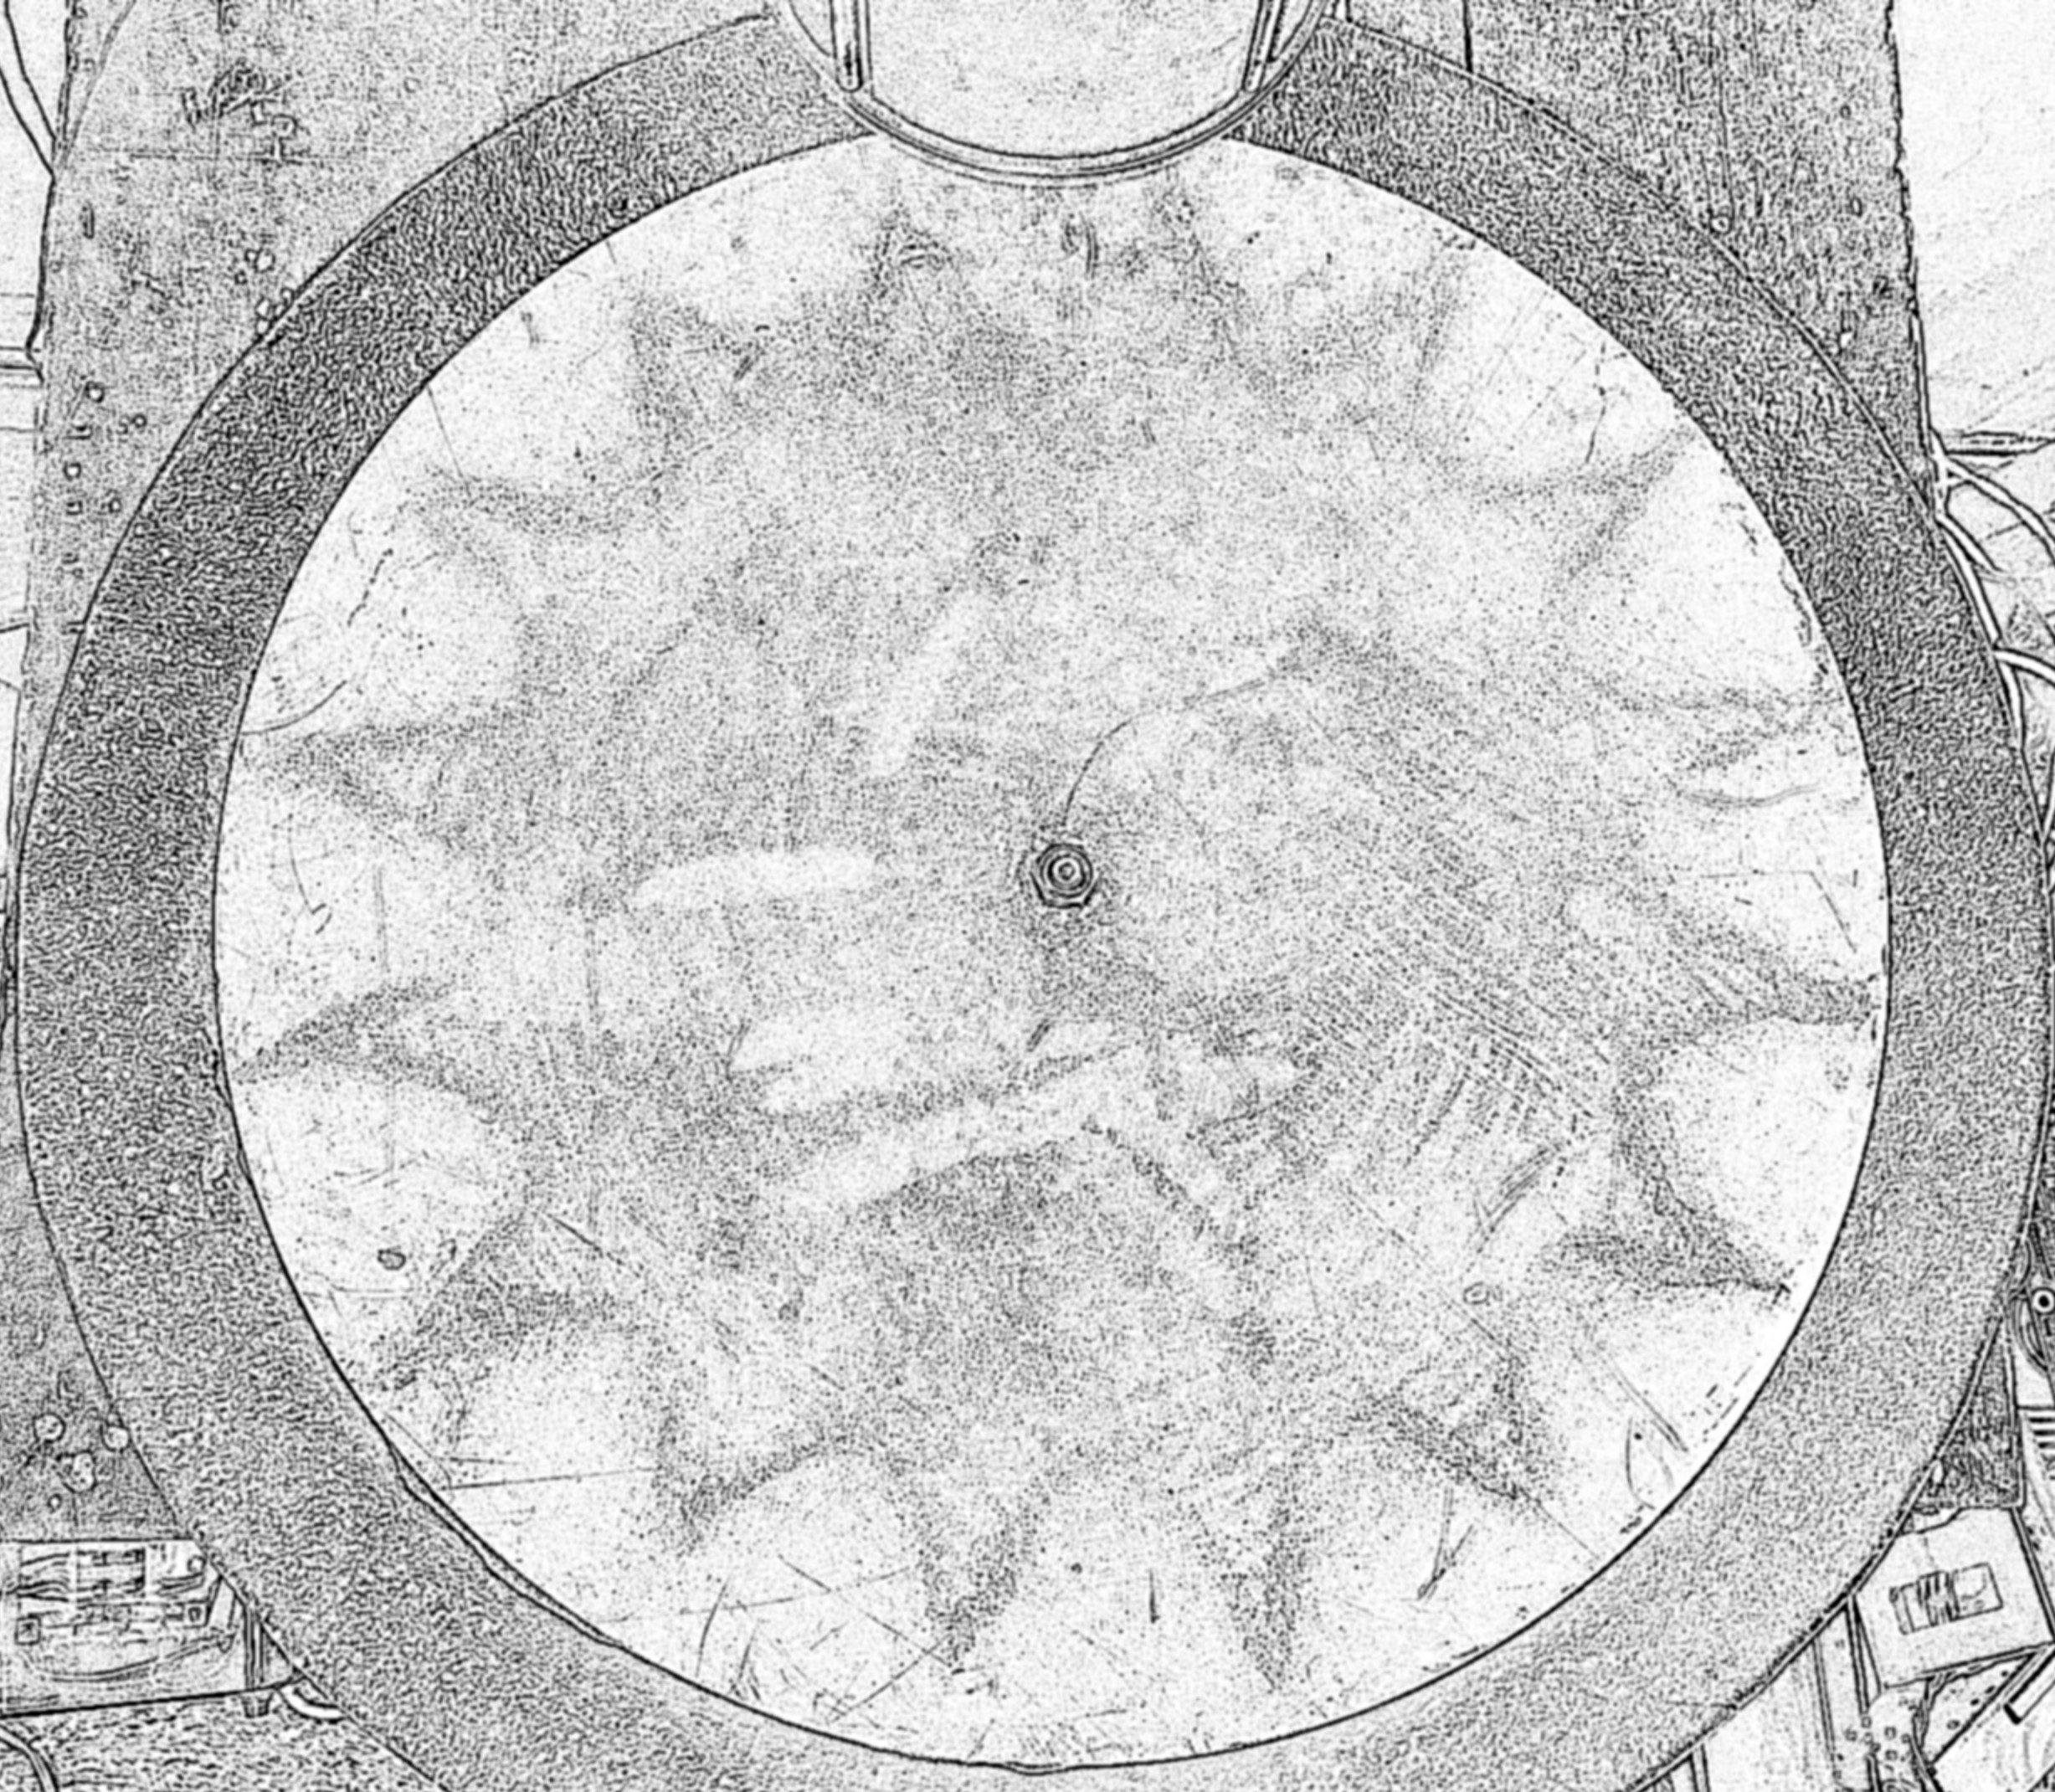
\includegraphics [height = 6cm] {Lab_7_Form_12.jpg} & 985 \\ [21ex]
        \hline
        13 & \center 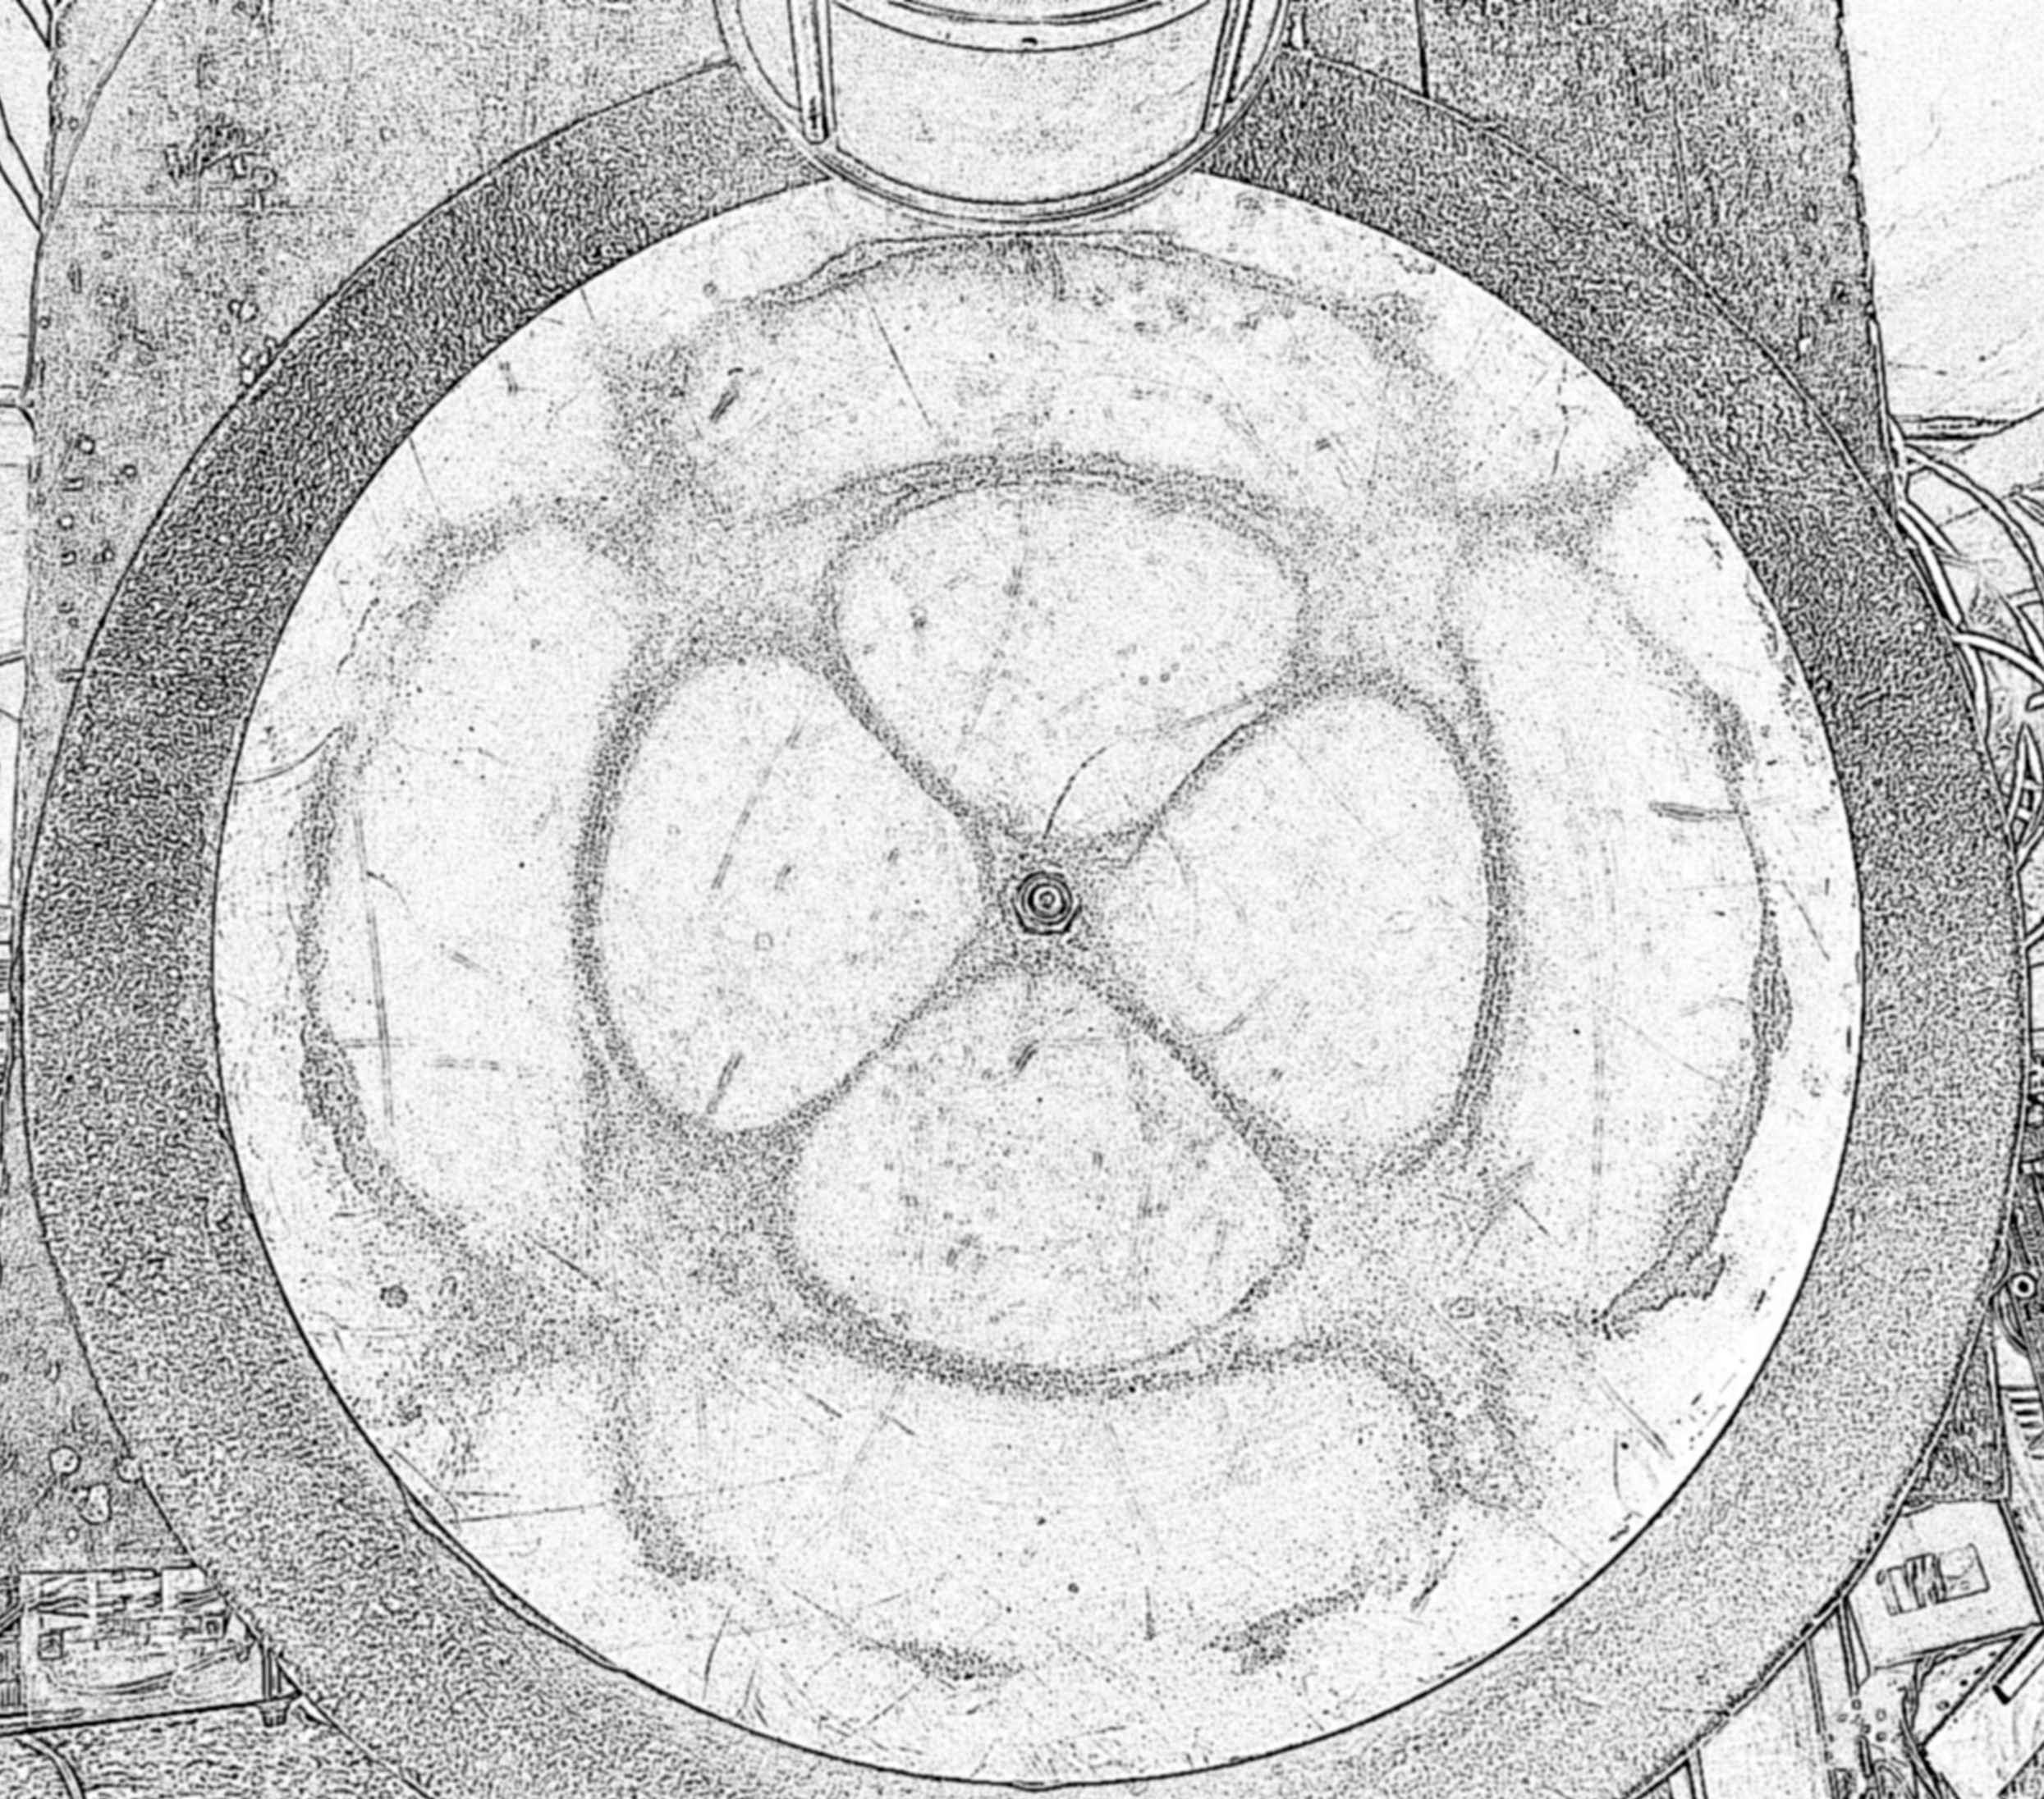
\includegraphics [height = 6cm] {Lab_7_Form_13.jpg} & 1050 \\ [21ex]
        \hline
        14 & \center 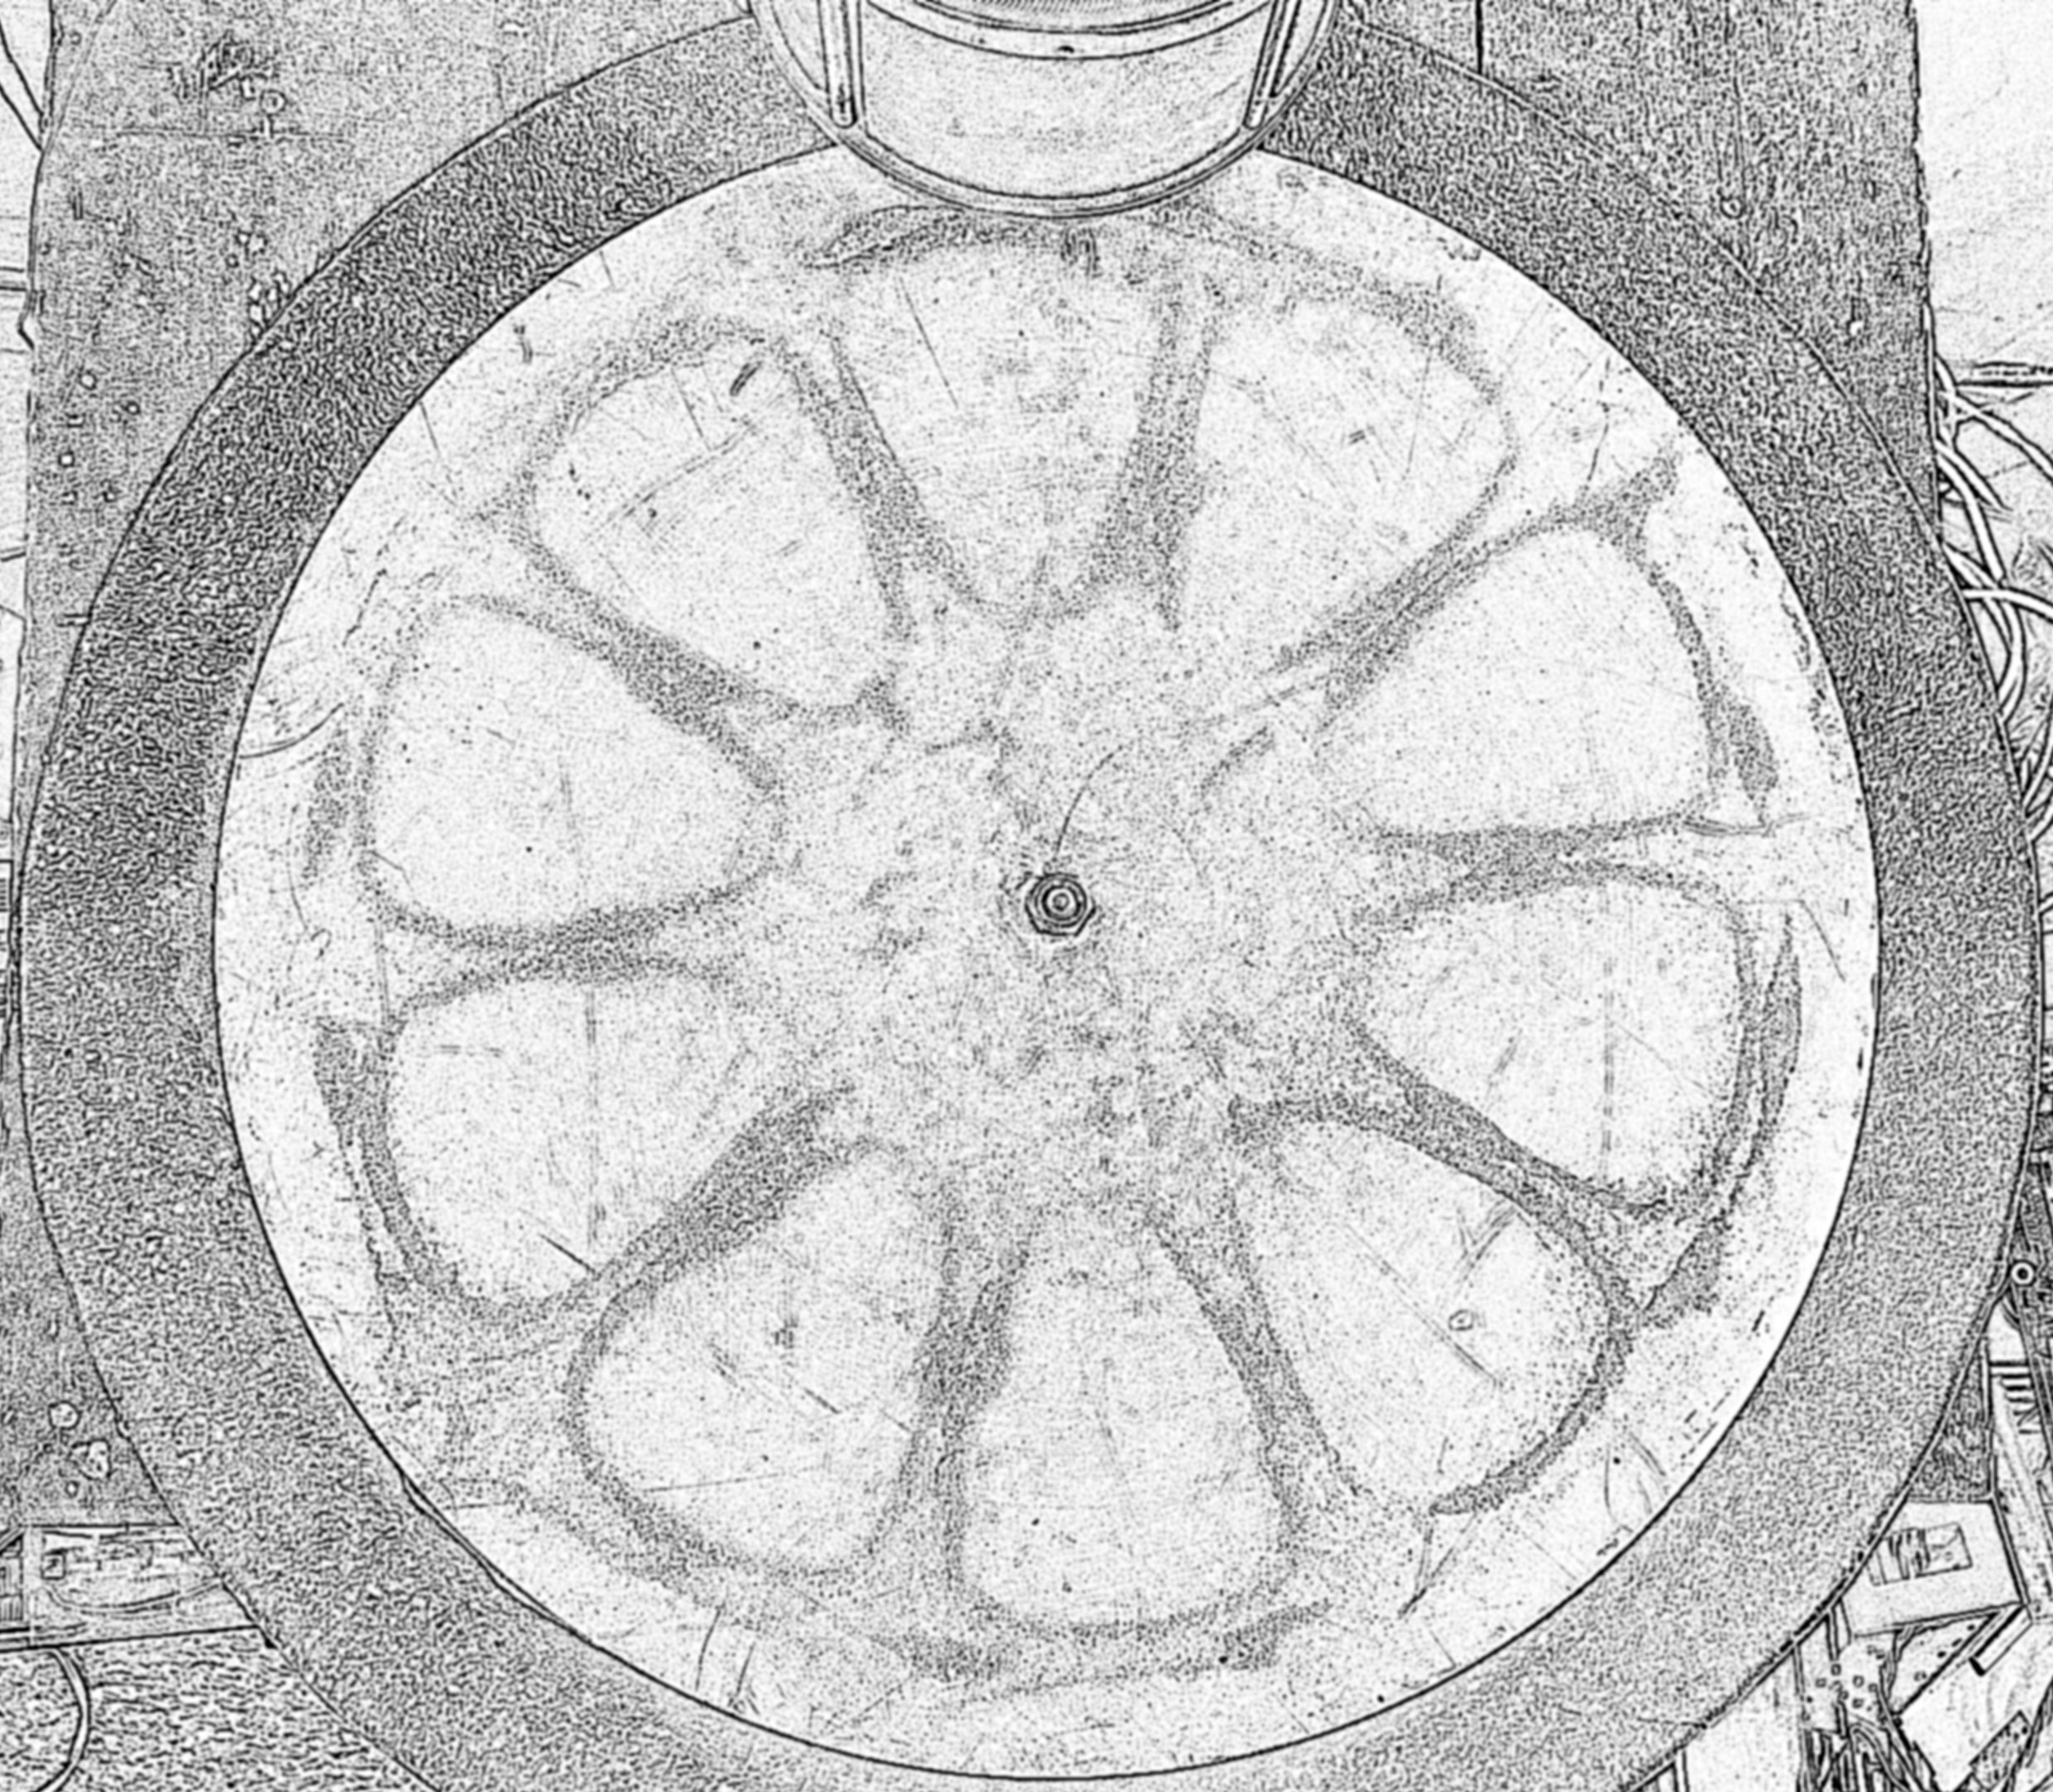
\includegraphics [height = 6cm] {Lab_7_Form_14.jpg} & 1175 \\ [21ex]
        \hline
        15 & \center 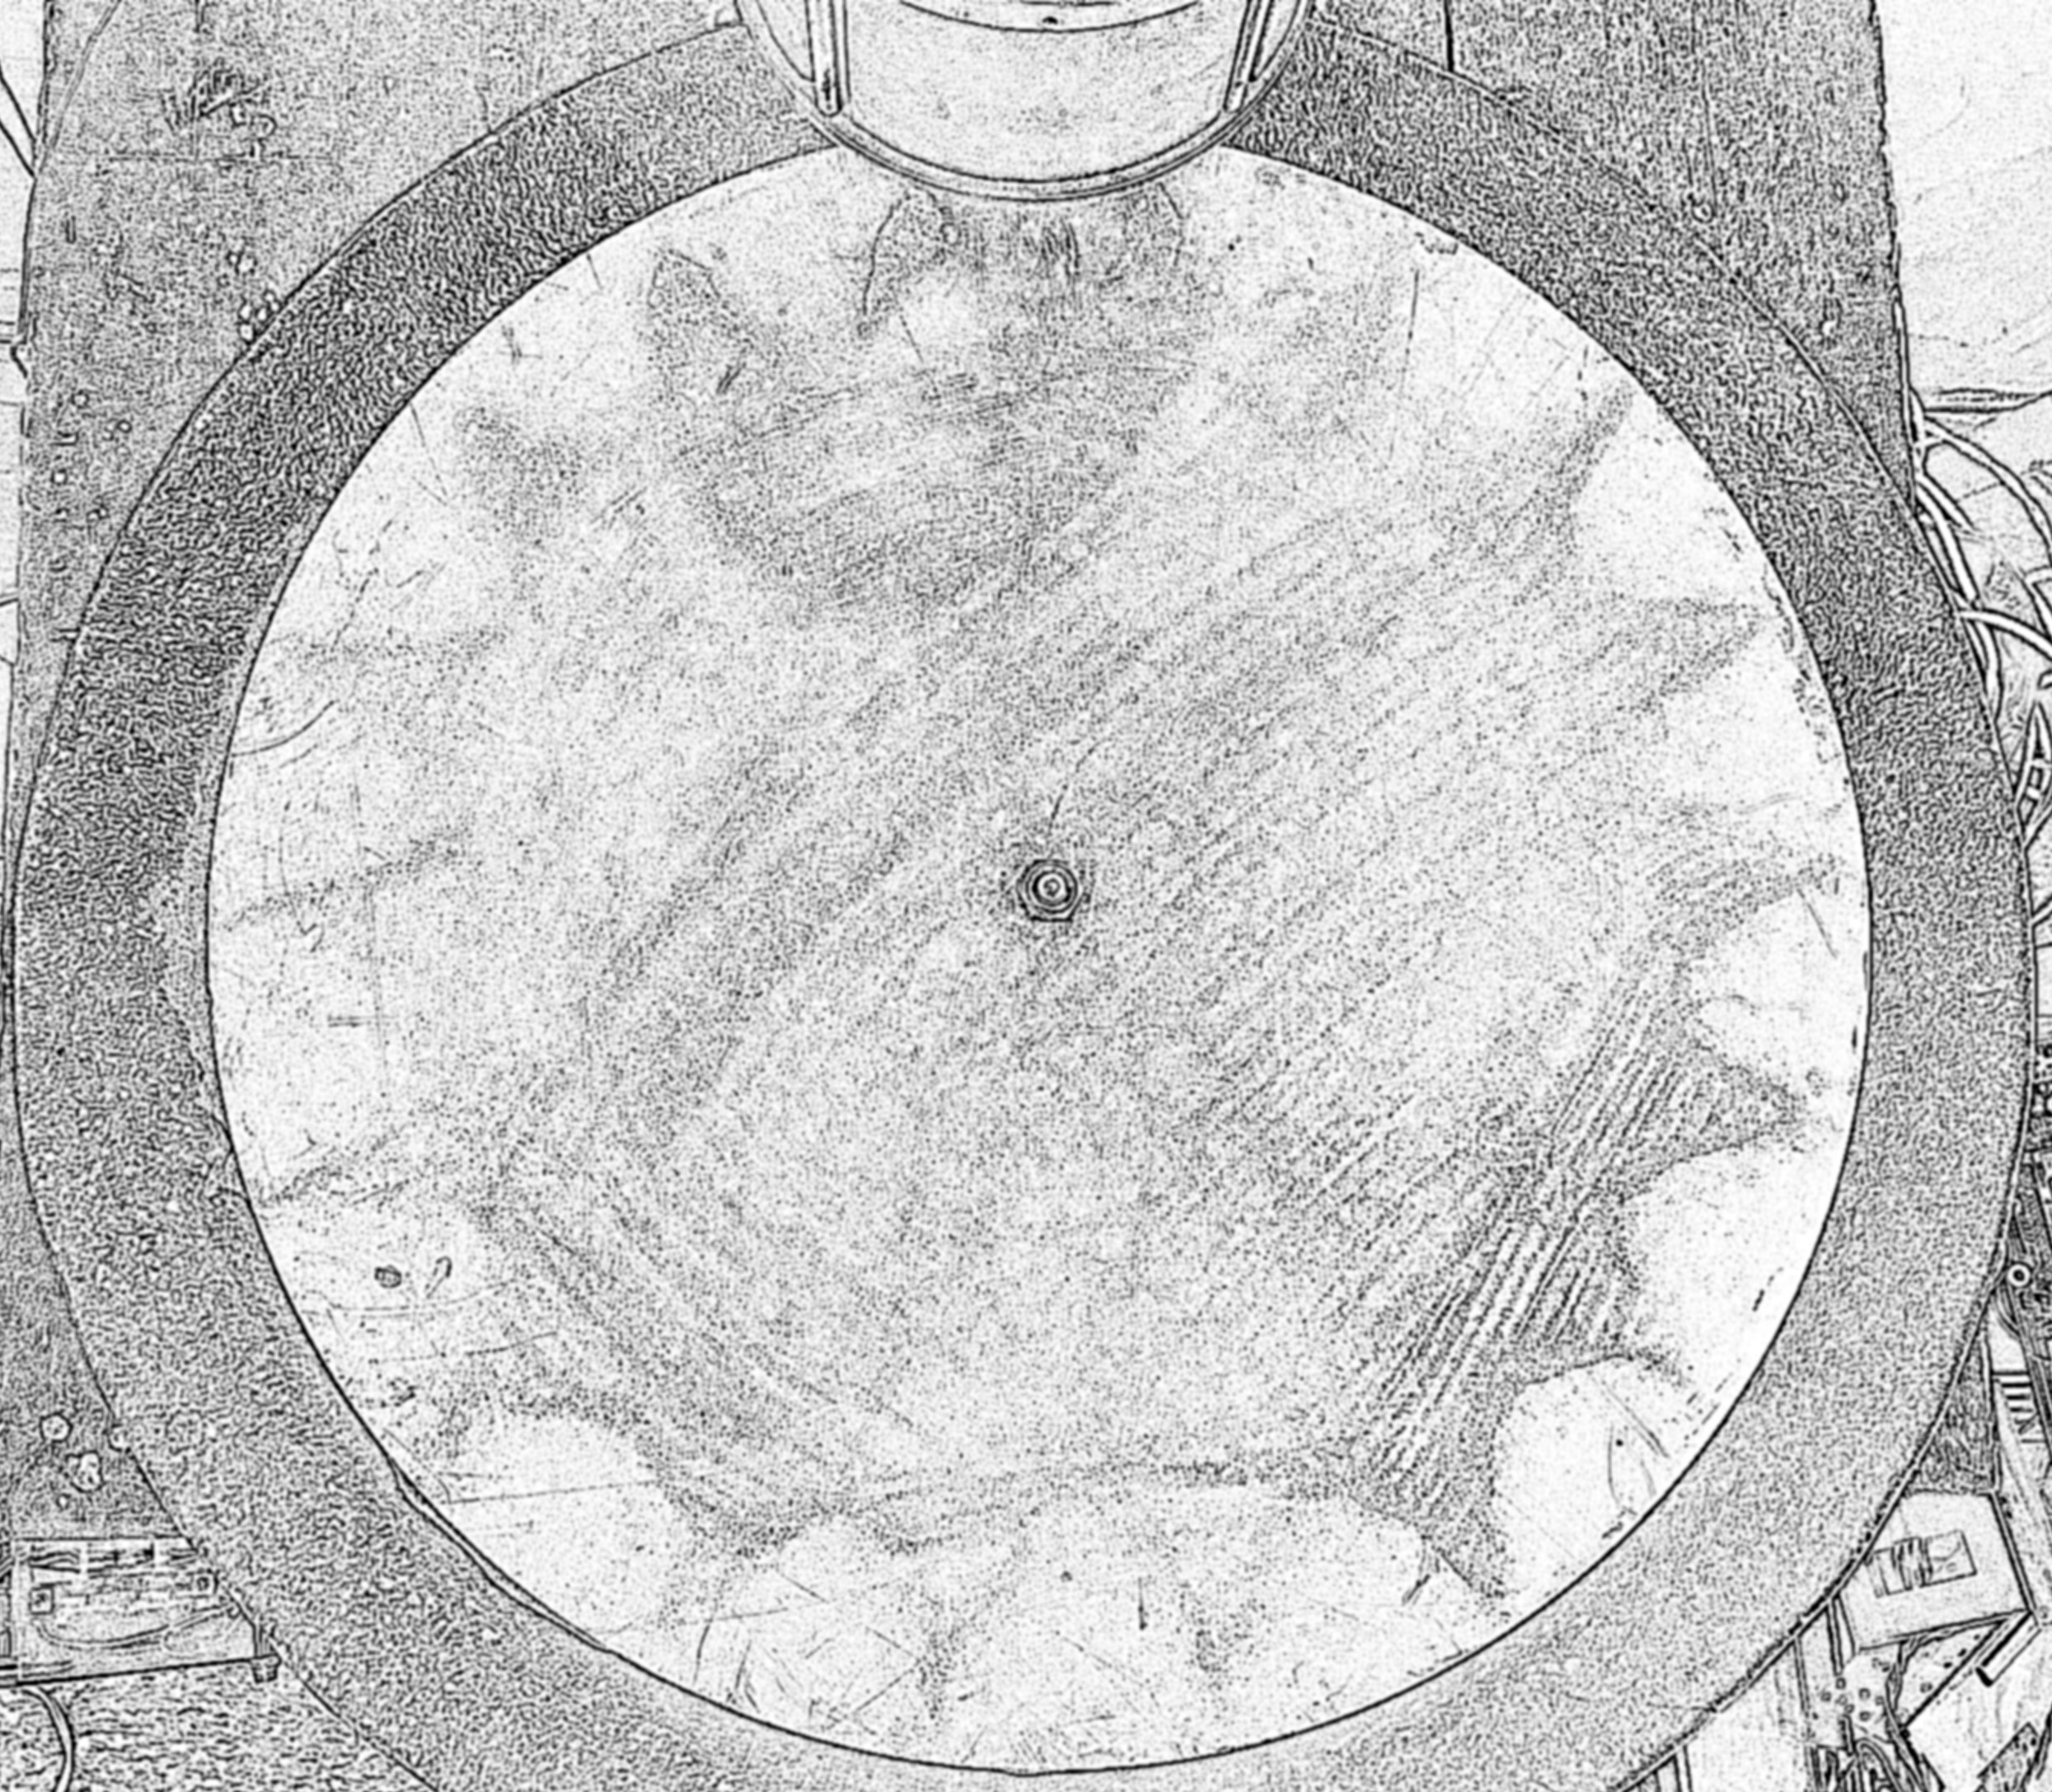
\includegraphics [height = 6cm] {Lab_7_Form_15.jpg} & 1225 \\ [21ex]
        \hline
        16 & \center 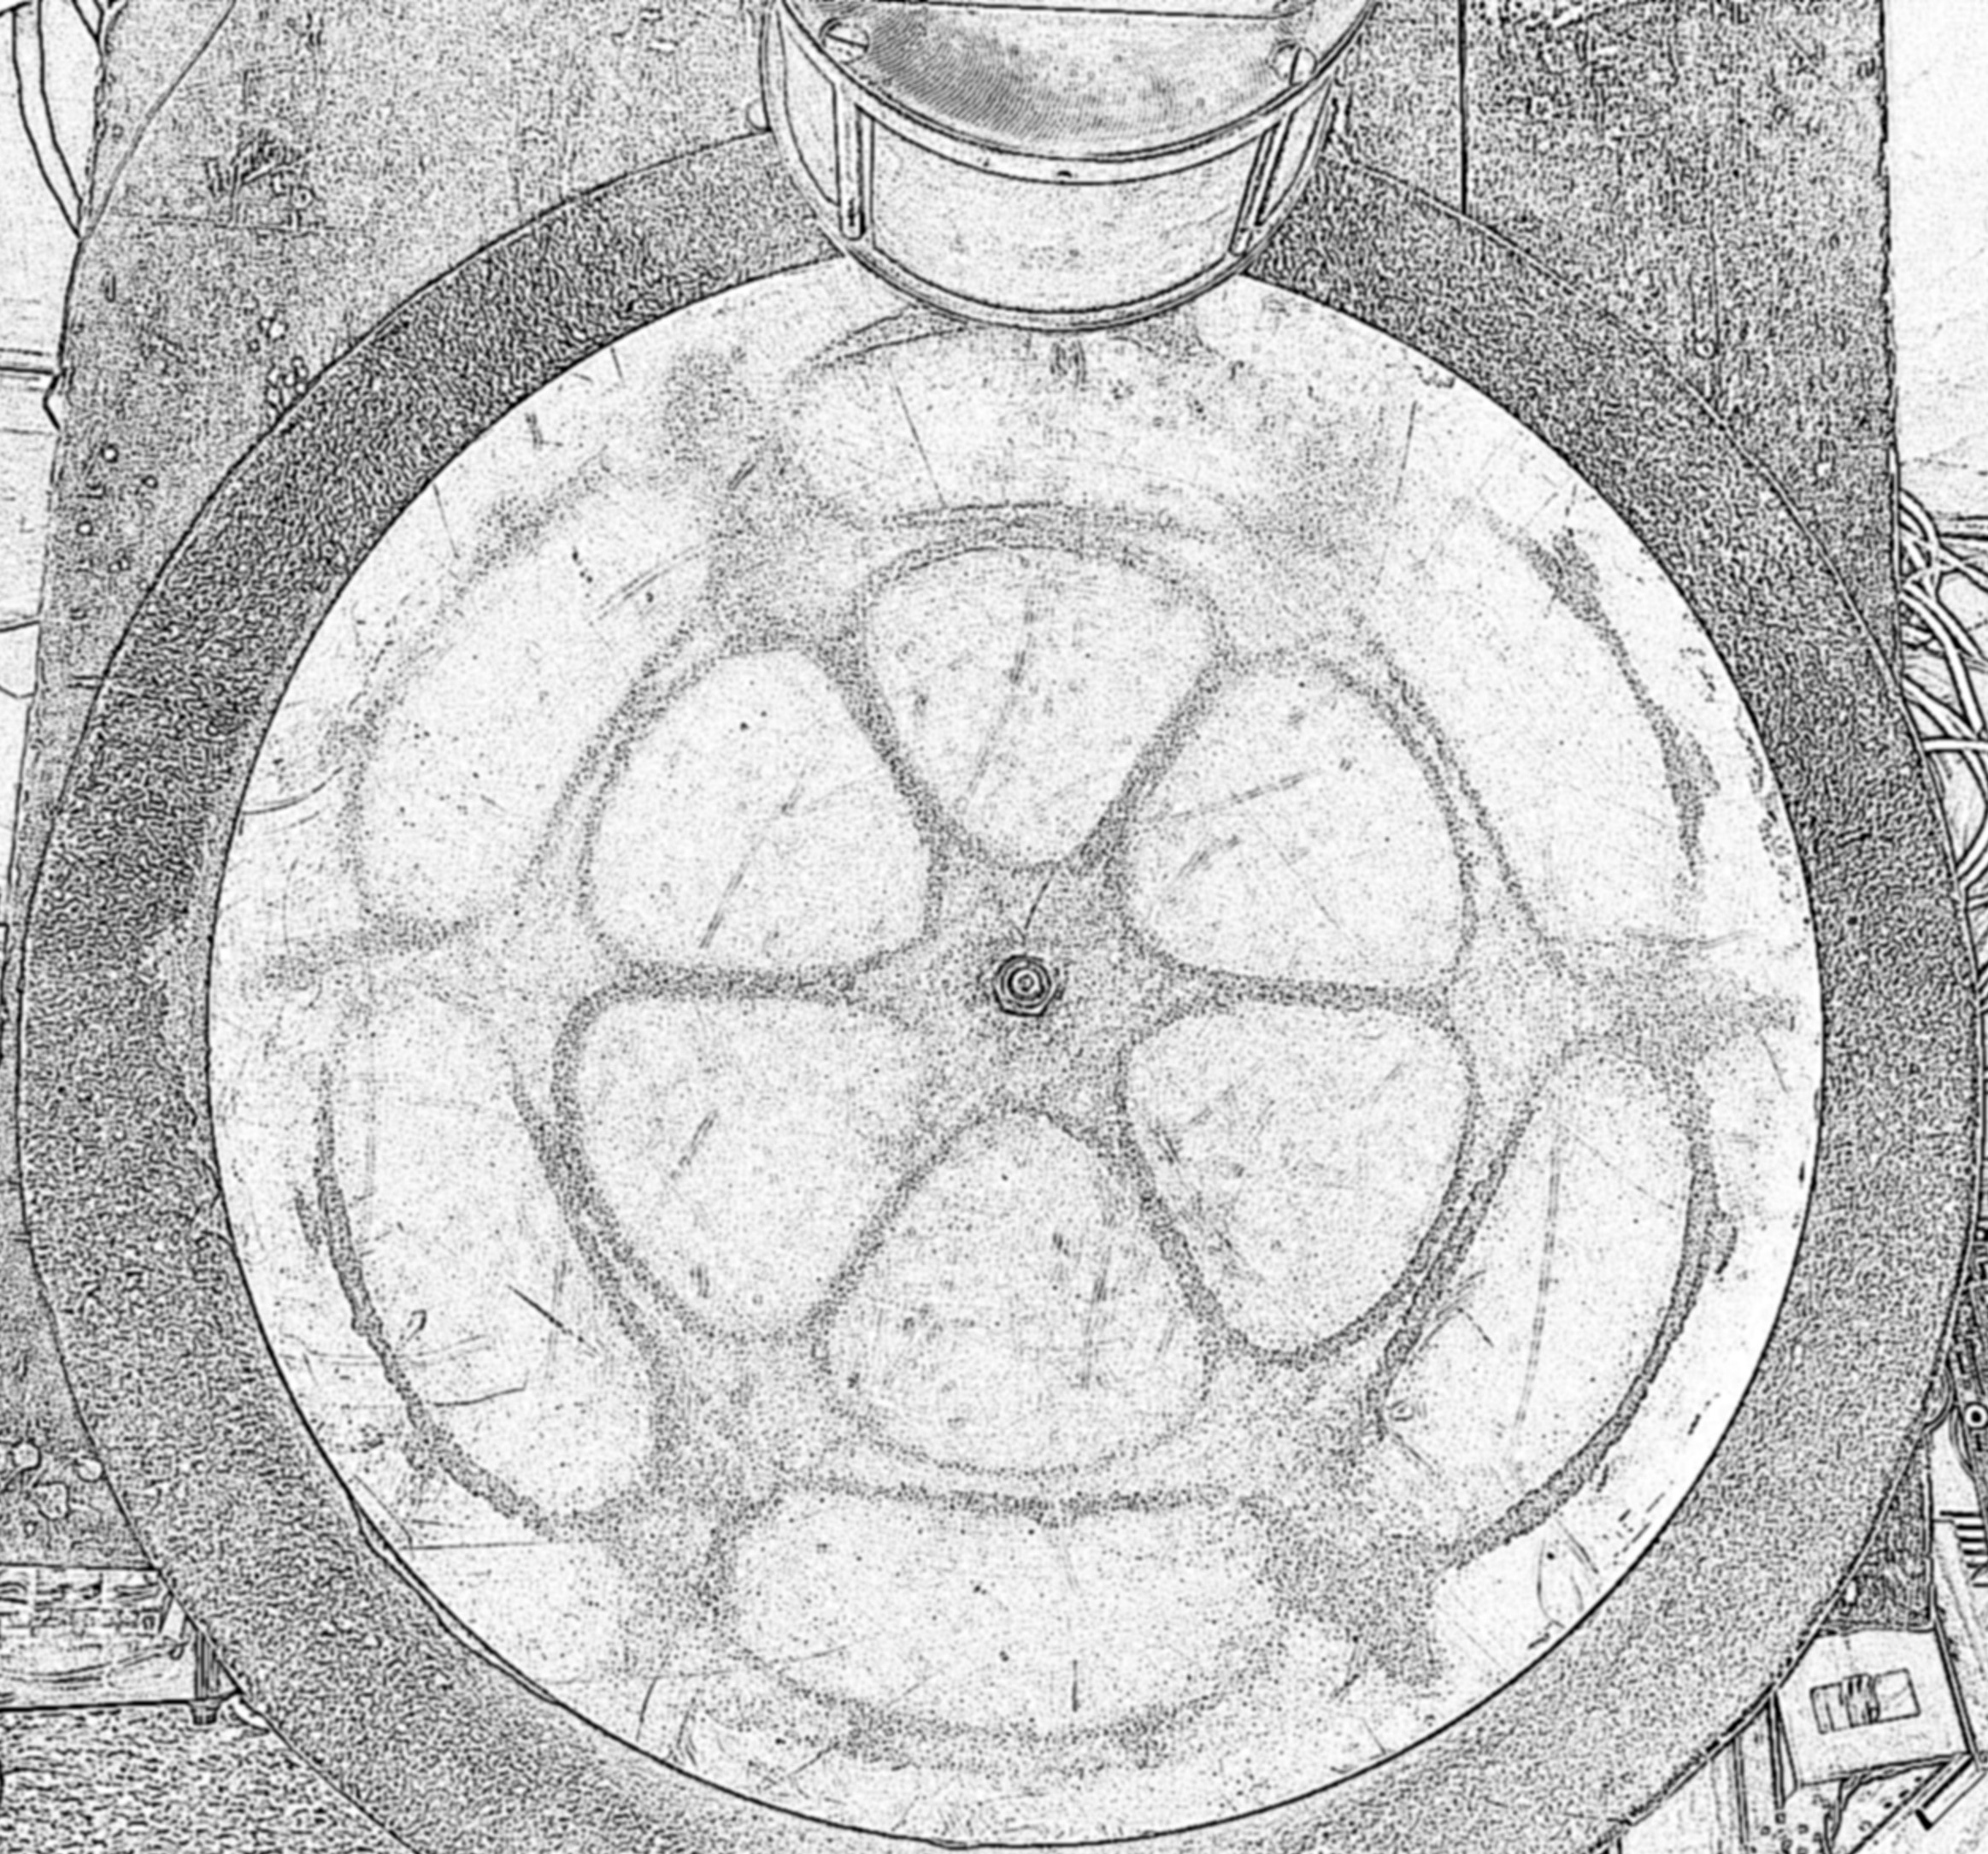
\includegraphics [height = 6cm] {Lab_7_Form_16.jpg} & 1360 \\ [21ex]
        \hline
        17 & \center 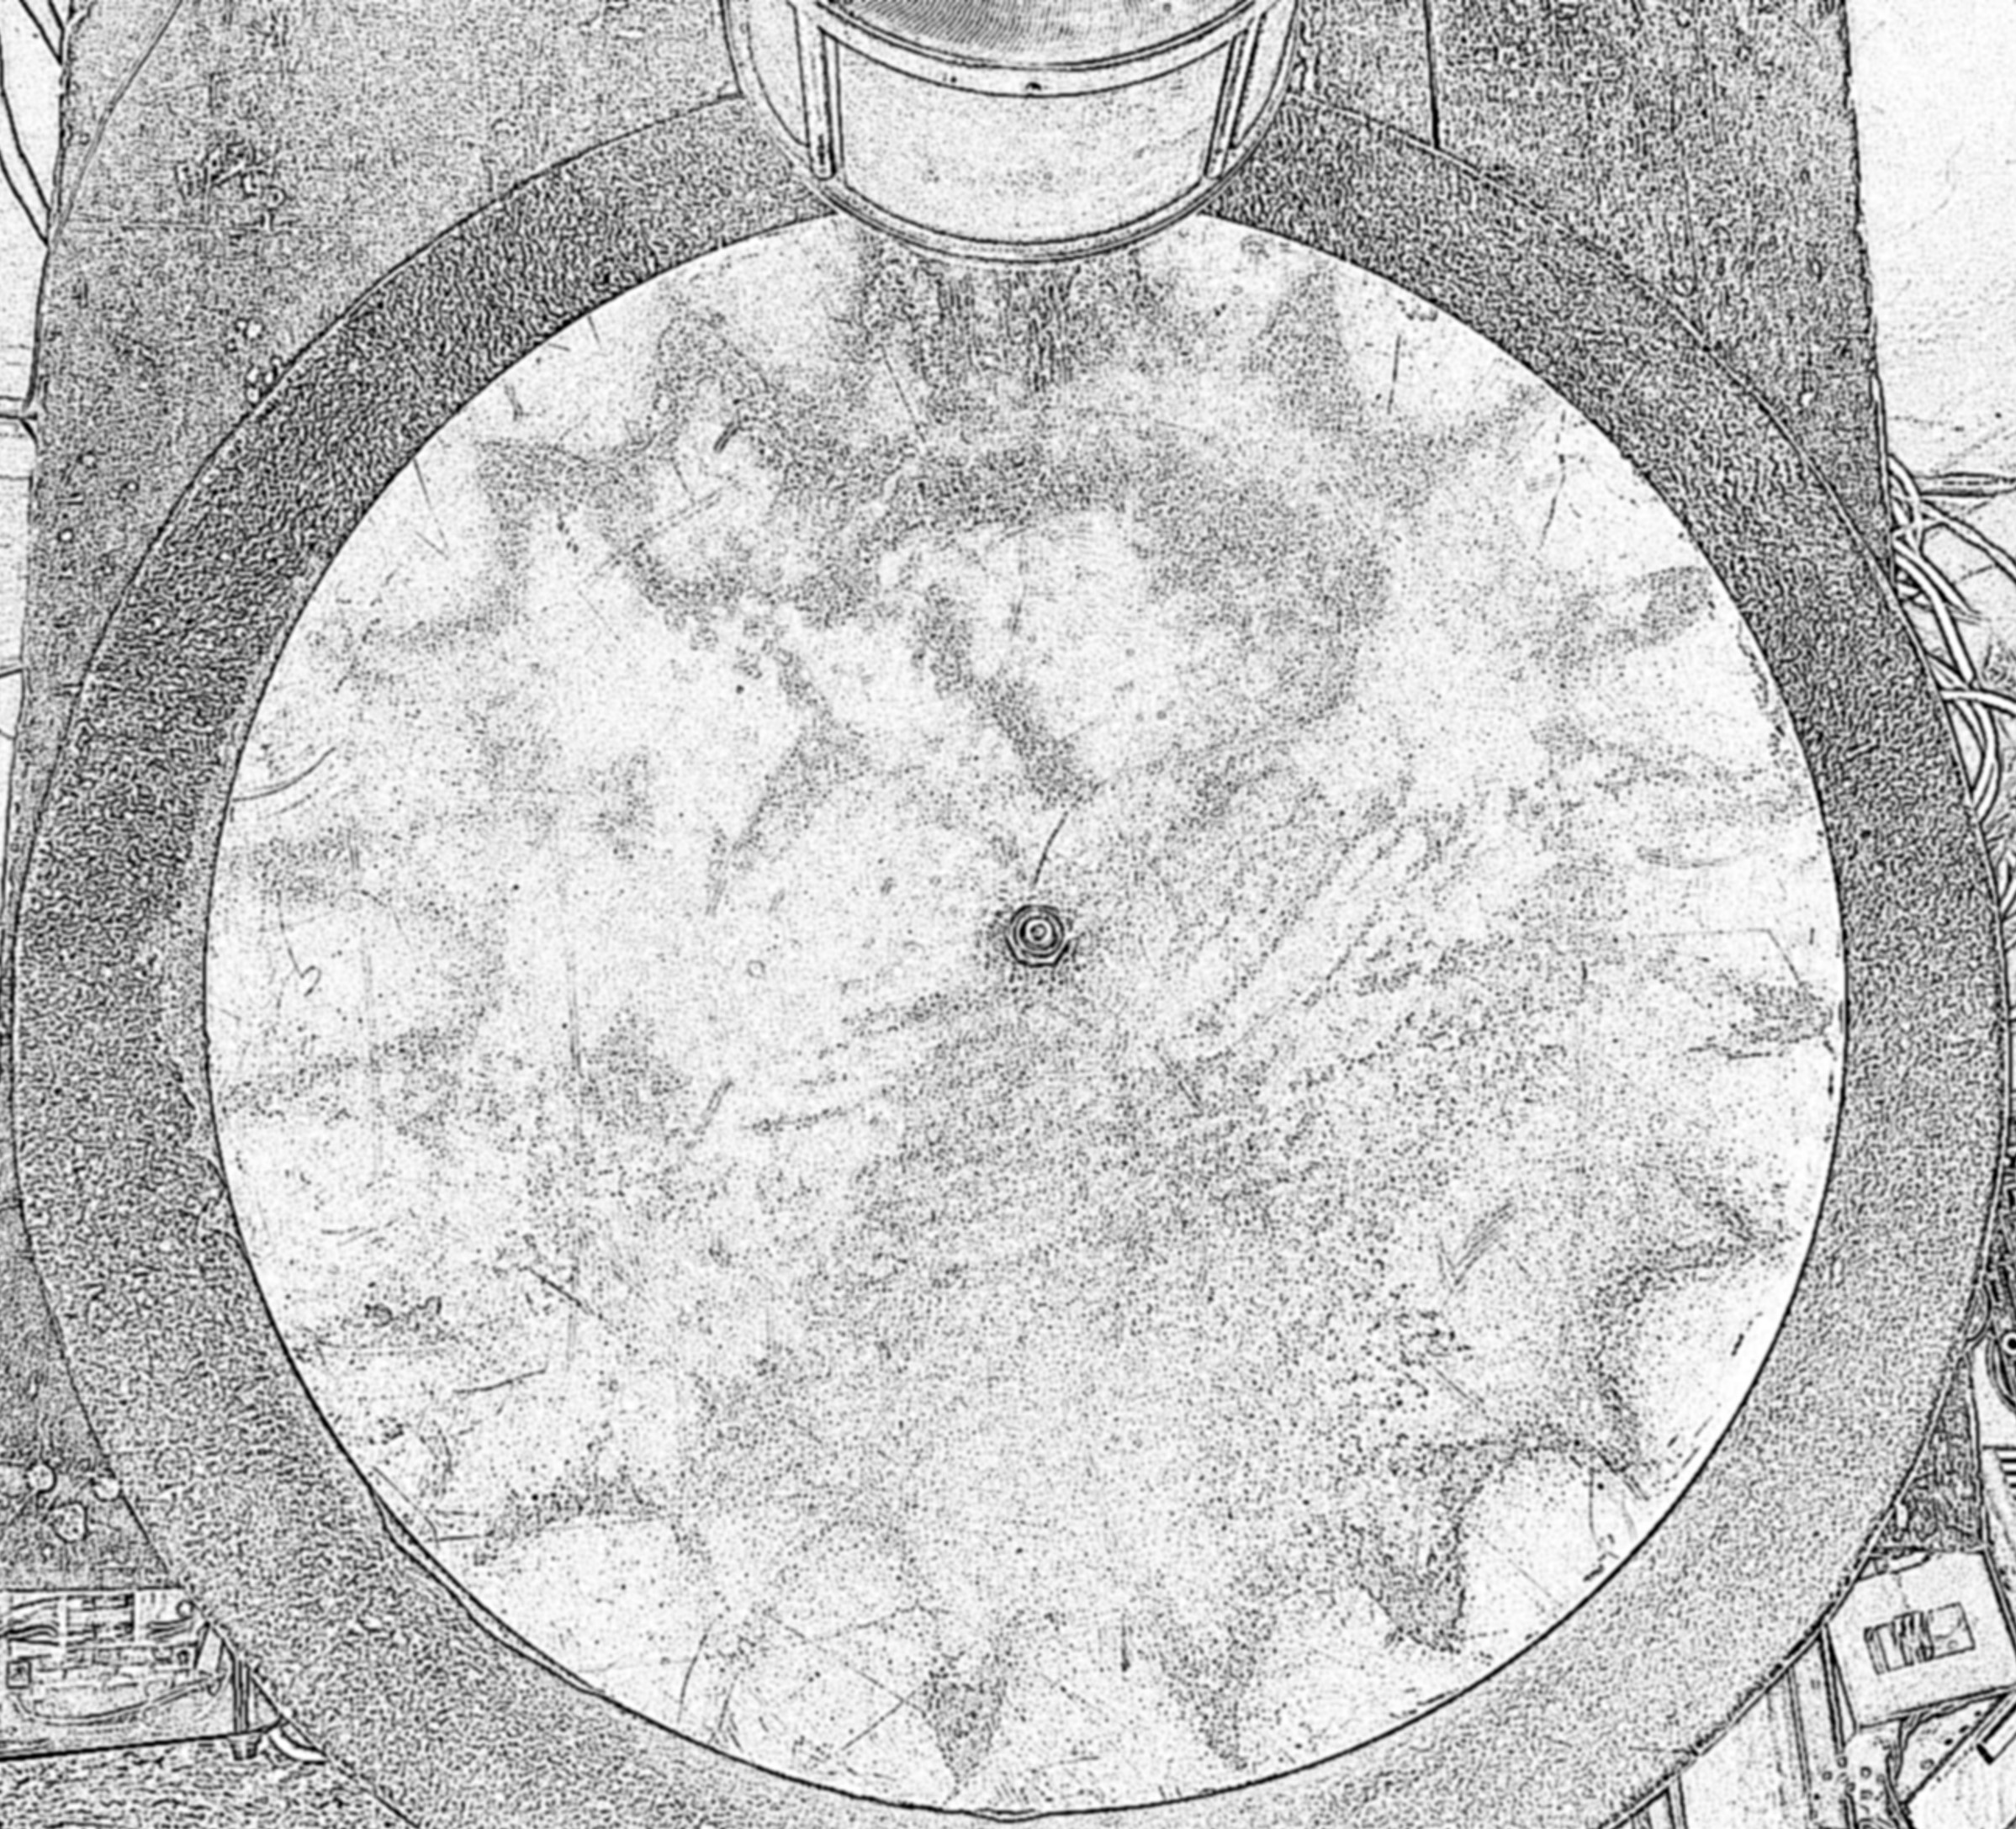
\includegraphics [height = 6cm] {Lab_7_Form_17.jpg} & 1500 \\ [21ex]
        \hline
        18 & \center 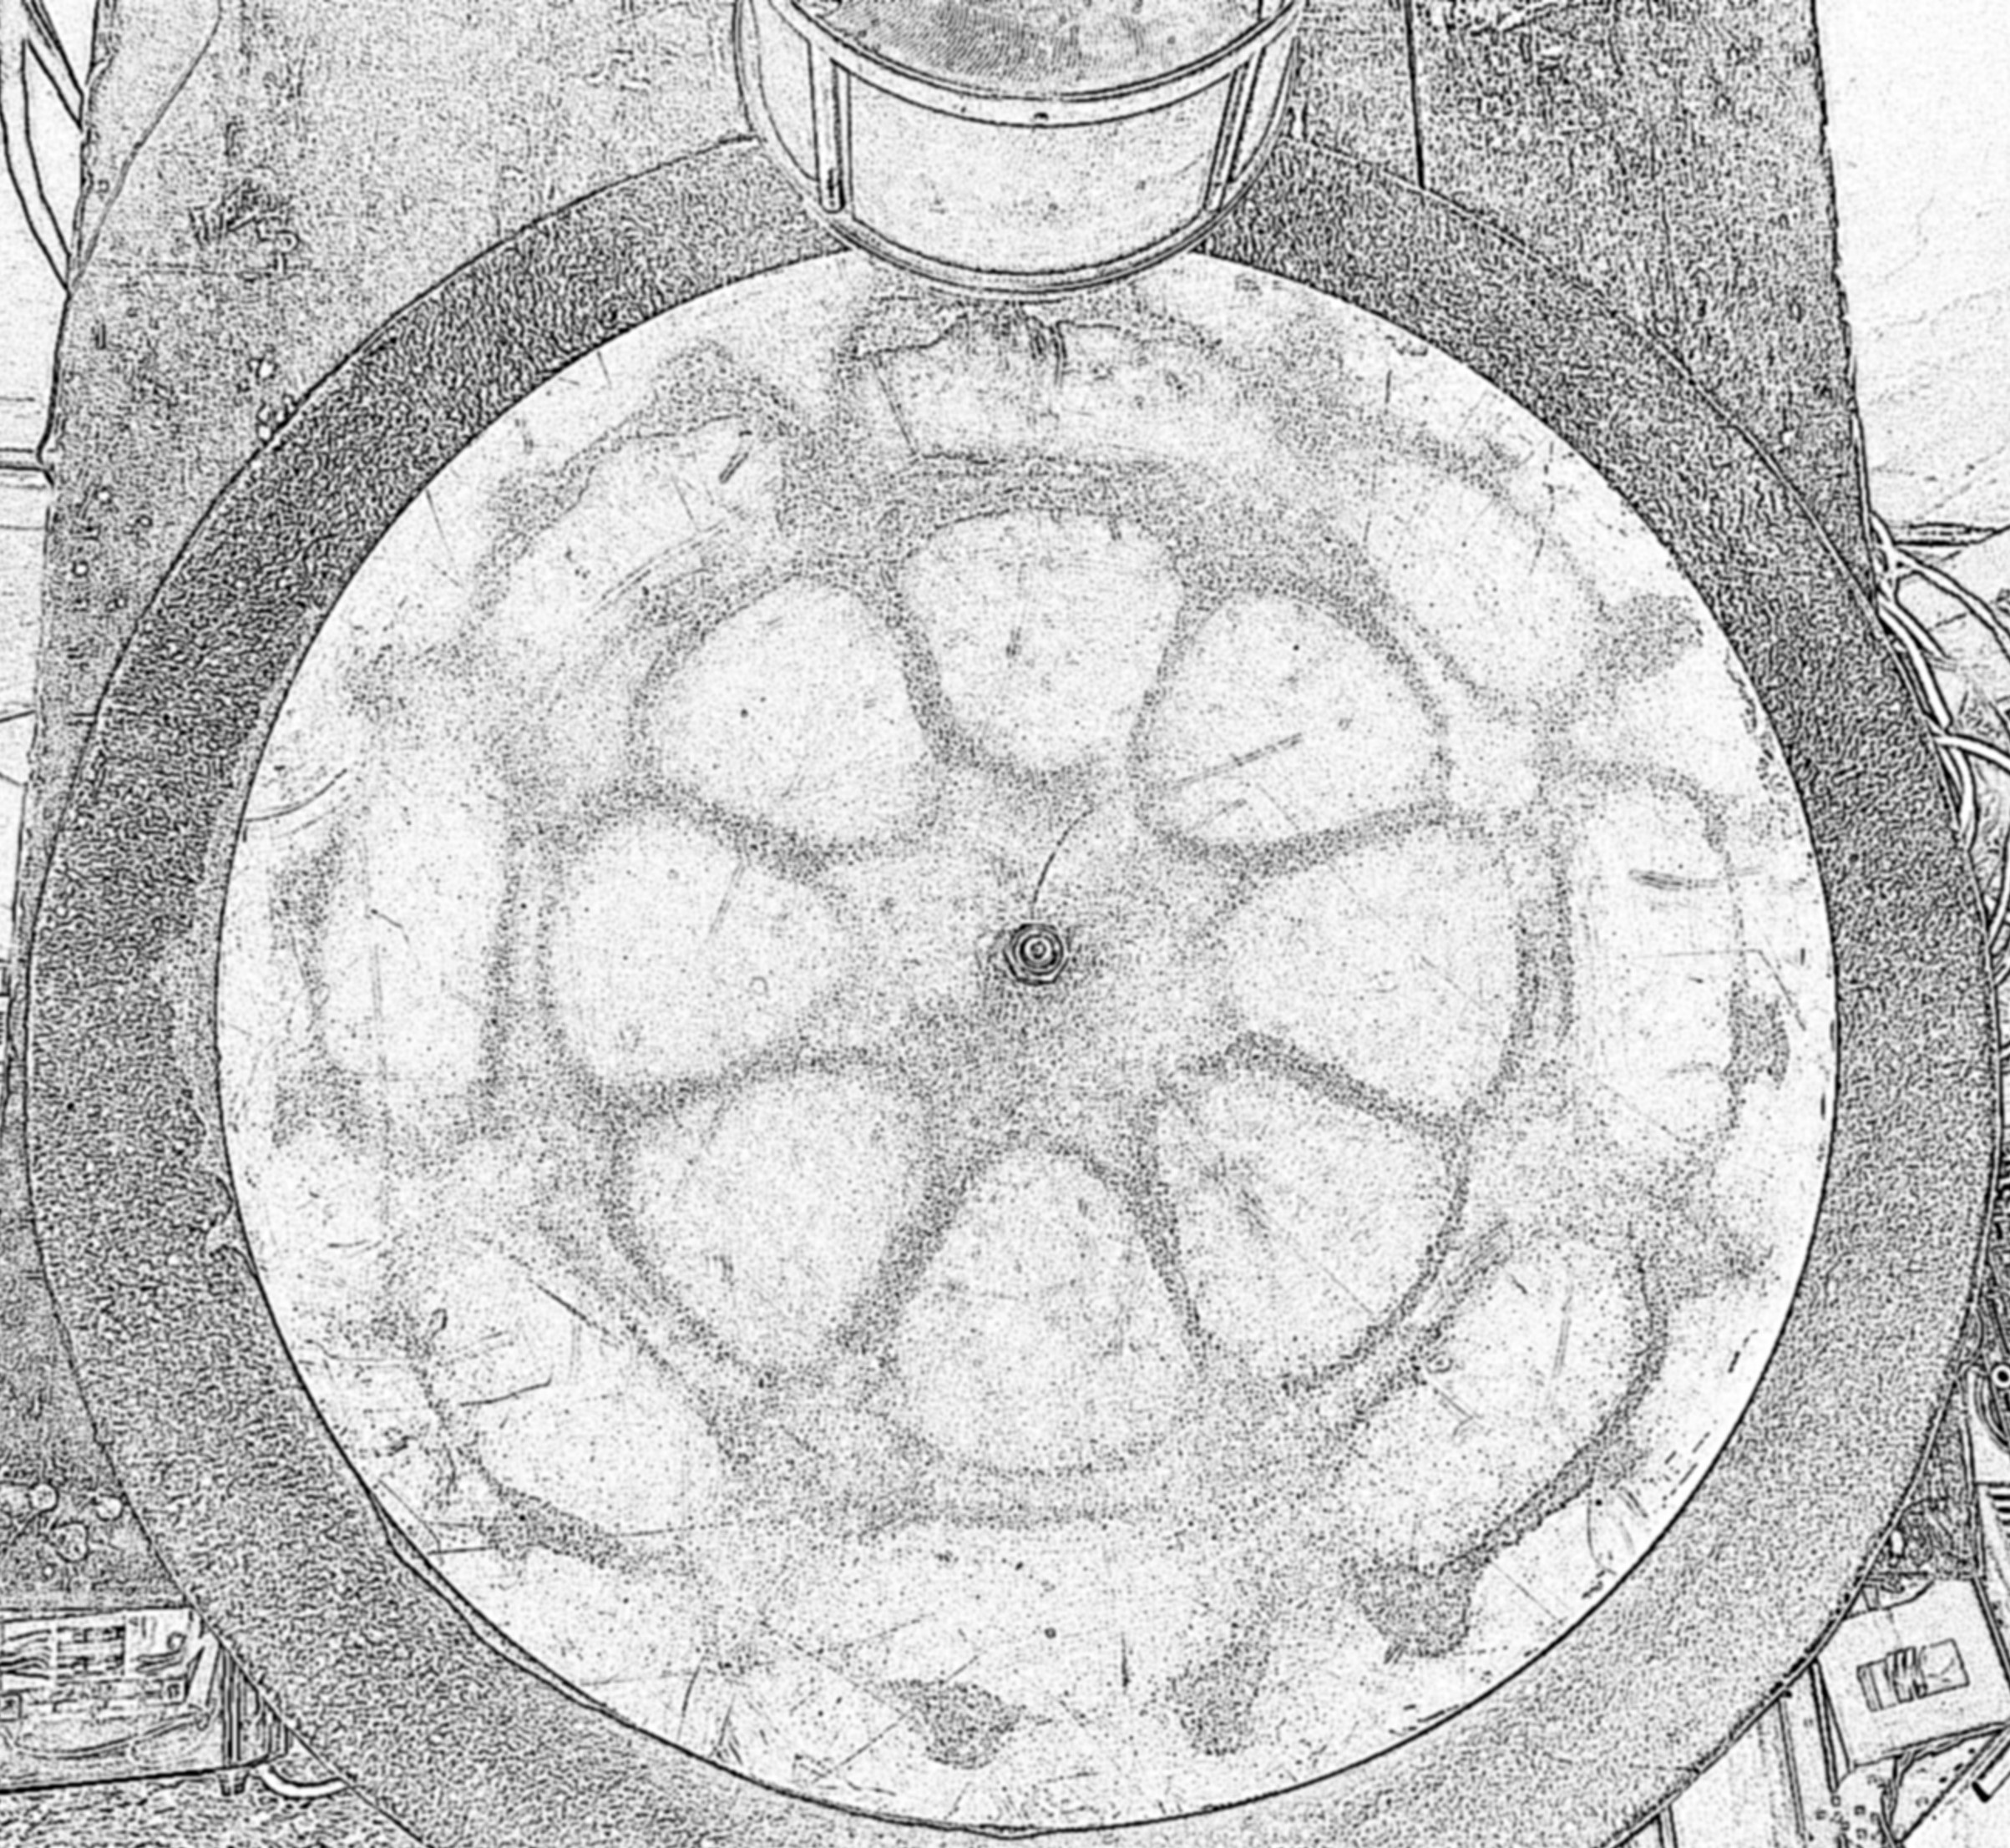
\includegraphics [height = 6cm] {Lab_7_Form_18.jpg} & 1730 \\ [21ex]
        \hline
    \end{longtable}
    
\end{document}